\documentclass[12pt, a4paper]{article}

\usepackage[utf8]{inputenc}
\usepackage[framemethod=TikZ]{mdframed}
\usepackage[hidelinks]{hyperref}
\usepackage{mathtools, amssymb, amsmath, cleveref, fancyhdr, geometry, graphicx, float, subfigure, arydshln, url, setspace, framed, pifont, physics, ntheorem, tcolorbox, utopia, multicol}
%%% for coding %%%
\usepackage{listings}
\usepackage[ruled, vlined, linesnumbered]{algorithm2e}

\geometry{a4paper, left=2cm, right=2cm, bottom=2cm, top=2cm}

\pagestyle{fancy}
\fancyhead{}
\fancyhead[L]{\leftmark}
\fancyhead[R]{\rightmark}
\fancyfoot{}
\fancyfoot[C]{\thepage}
%\renewcommand{\headrulewidth}{0pt}
\renewcommand{\footrulewidth}{0pt}

\hypersetup{
	colorlinks = true,
	bookmarks = true,
	bookmarksnumbered = true,
	pdfborder = 001,
	linkcolor = blue
}

\definecolor{grey}{rgb}{0.49,0.38,0.29}
\definecolor{mygreen}{rgb}{0,0.6,0}


%%% for coding %%%
\lstset{basicstyle = \ttfamily\small,commentstyle = \color{mygreen}\textit, deletekeywords = {...}, escapeinside = {\%*}{*)}, frame = single, framesep = 0.5em, keywordstyle = \bfseries\color{blue}, morekeywords = {*}, emph = {self}, emphstyle=\bfseries\color{red}, numbers = left, numbersep = 1.5em, numberstyle = \ttfamily\small\color{grey},  rulecolor = \color{black}, showstringspaces = false, stringstyle = \ttfamily\color{purple}, tabsize = 4, columns = flexible}

\newcounter{index}[subsection]
\setcounter{index}{0}
\newenvironment*{df}[1]{\par\noindent\textbf{Definition \thesubsection.\stepcounter{index}\theindex\ (#1).}}{\par}

\newenvironment*{eg}[1]{\begin{framed}\par\noindent\textbf{Example \thesubsection.\stepcounter{index}\theindex\ #1} \par}{\par\end{framed}}

\newenvironment*{thm}[1]{\begin{tcolorbox}\par\noindent\textbf{Theorem \thesubsection.\stepcounter{index}\theindex\ #1} \par}{\par\end{tcolorbox}}

\newenvironment*{cor}[1]{\par\noindent\textbf{Corollary \thesubsection.\stepcounter{index}\theindex\ #1}}{\par}
\newenvironment*{lem}[1]{\par\noindent\textbf{Lemma \thesubsection.\stepcounter{index}\theindex\ #1}}{\par}
\newenvironment*{ax}[1]{\par\noindent\textbf{Axiom \thesubsection.\stepcounter{index}\theindex\ #1}}{\par}
\newenvironment*{prop}[1]{\par\noindent\textbf{Proposition \thesubsection.\stepcounter{index}\theindex\ #1}}{\par}
\newenvironment*{conj}[1]{\par\noindent\textbf{Conjecture \thesubsection.\stepcounter{index}\theindex\ #1}}{\par}
\newenvironment*{nota}{\par\noindent\textbf{Notation \thesubsection.\stepcounter{index}\theindex.}}{\par}


\newcounter{nprf}[subsection]
\setcounter{nprf}{0}
\newenvironment*{prf}{\par\indent\textbf{\textit{Proof \stepcounter{nprf}\thenprf.}}}{\hfill$\blacksquare$\par}
\newenvironment*{dis}{\par\indent\textbf{\textit{Disproof \stepcounter{nprf}\thenprf.}}}{\hfill$\blacksquare$\par}
\newenvironment*{sol}{\par\indent\textbf{\textit{Solution \stepcounter{nprf}\thenprf.}}\par}{\hfill{$\square$}\par}

\newtheorem{hint}{Hint.}[section]
\newtheorem{rmk}{Remark.}[section]
\newtheorem{ext}{Extension.}[section]
\newtheorem{clm}{Claim.}[section]

\linespread{1.25}

\title{\textbf{Emory University\\\textbf{MATH 315 Numerical Analysis}\\ Learning Notes}}
\author{Jiuru Lyu}
\date{\today}

\def\Z{{\mathbb{Z}}}
\def\R{{\mathbb{R}}}
\def\C{{\mathbb{C}}}
\def\Q{{\mathbb{Q}}}
\def\E{{\mathbb{E}}}
\def\d{{\mathrm{d}}}
\def\float{\texttt{float}}
\def\flt{\texttt{float}}
\def\Inf{\texttt{Inf}}
\def\NaN{\texttt{NaN}}
\def\epsilon{\varepsilon}
\def\phi{\varphi}
\def\emptyset{\varemptyset}
\def\A{\vb A}
\def\dsst{\displaystyle}
\def\bigO{\mathcal{O}}
\def\pqed{\quad\square}
\def\st{\emph{\ s.t.\ }}
\def\hat{\widehat}
\def\tilde{\widetilde}
\def\l{\ell}
\def\DOP{\mathrm{DOP}}

\begin{document}
\maketitle

\tableofcontents

\newpage
\section{Floating Point Numbers}
\subsection{Binary Representation}
\begin{df}{Binary}
	$0$ and $1$; on and off.	
\end{df}
\begin{eg}{Represent Numbers in Base-2}
	\par Consider $13=1(10)+3(1)=1(10)+3(10^0)$ in base-10. It can be converted into base-2 by decomposing $13$ as $1(2^3)+1(2^2)+0(2^1)+1(2^0)$.
\end{eg}
\begin{eg}{Fractions in Base-2}
	\[\dfrac{7}{16}=\dfrac{1}{16}(7)=\qty(2^{-4})\qty(2^2+2^1+2^0)=2^{-2}+2^{-3}+2^{-4}.\]
\end{eg}
\begin{eg}{Repeating Fractions in Base-2}
	\[\begin{aligned}\dfrac{1}{5}=\dfrac{1}{8}+\epsilon_1\quad&\Longrightarrow\quad\epsilon_1=\dfrac{1}{5}-\dfrac{1}{8}=\dfrac{8-5}{(5\times8)}=\dfrac{3}{40}\\\epsilon_1=\dfrac{3}{3(16)}+\epsilon_2\quad&\Longrightarrow\quad\cdots\end{aligned}\] Repeating the steps above, we would finally get \[\dfrac{1}{5}=\dfrac{1}{8}+\dfrac{1}{16}+\dfrac{1}{128}+\dfrac{1}{256}+\cdots\]
\end{eg}
\begin{thm}{}
	Let $n\in\Z$ and $n\geq1$, then \[\sum_{k=0}^{n-1}2^k=2^{n-1}+2^{n-2}+\cdots+2^0=2^n-1.\]	
\end{thm}
\subsection{Integers in Computers}
\begin{df}{Storing Integers}
	\texttt{unit8} stands for unsigned integers and \texttt{int8} stands for signed integers. 
	\begin{rmk} The $8$ here represents $8$ bits. It is a measure of how much storage (how many $0$s or $1$s).\end{rmk}
	\[\begin{aligned}
	\begin{tabular}{|c|c|c|c|c|c|c|c|}
		\hline
		\ $b_7$&$b_6$\ &\ $b_5$&$b_4$\ &\ $b_3$&$b_2$\ &\ $b_1$&\ $b_0$\\
		\hline
	\end{tabular}&\\
	\begin{tabular}{ccccccccc}	
		unsigned: &$2^7$&$2^6$&$2^5$&$2^4$&$2^3$&$2^2$&$2^1$&$2^0$\\
		signed:   &$-2^7$&$2^6$&$2^5$&$2^4$&$2^3$&$2^2$&$2^1$&$2^0$
	\end{tabular}&
	\end{aligned}\]
\end{df}
\begin{eg}{}
	\[\texttt{unit8}(13)=00001101\] Since $-13=1(-2^7)+1(2^6)+1(2^5)+1(2^4)+0(2^3)+0(2^2)+1(2^1)+1(2^0)$, we have \[\texttt{int8}(-13)=11110011\]
\end{eg}
\begin{rmk}
	Largest and Smallest Integers: \[\begin{aligned}\textnormal{\texttt{uint8}}(x_L)&=11111111\quad\Longrightarrow x_L=2^7+2^6+\cdots+2^0=2^8-1=255\\\textnormal{\texttt{uint8}}(x_S)&=00000000\quad\Longrightarrow x_S=0(2^7)+0(2^6)+\cdots+0(2^0)=0\\\textnormal{\texttt{int8}}(x_L)&=01111111\quad\Longrightarrow x_L=0(-2^7)+2^6+\cdots+2^0=2^7-1=127\\\textnormal{\texttt{int8}}(x_S)&=100000000\quad\Longrightarrow x_S=1(-2^7)+0(2^6)+\cdots+0(2^0)=-128\end{aligned}\]	
\end{rmk}
\subsection{Representation of Floating Point Numbers}
\begin{df}{Normalized Scientific Notation}
	Only $1$ digit (non-zero) to the left of the decimal point.	
\end{df}
\begin{eg}{}
	\[\begin{aligned}123.456\times10^7&\\12.3456\times10^8&\\1.23456\times10^9&\rightarrow\text{normalized}\end{aligned}\]	
\end{eg}
\begin{df}{Anatomy of Floating Point Numbers}
	A floating point number, $\texttt{float}(x)$, consists of three parts: $s(x)$ (sign bit), $e(x)$ (exponent bits), and $f(x)$ (fraction bits).
\end{df}
\begin{df}{Precision}
	Precision is defined by the number 	of bits per part:
	\begin{center}\begin{tabular}{c|c|c|c|c}
	&$s(x)$&$e(x)$&$f(x)$&total\\\hline
	double precision (DP)&$1$&$11$&$52$&$64$\\
	single precision (SP)&$1$&$8$&$23$&$32$\\
	half precision (HP)&$1$&$5$&$10$&$16$\\
	\end{tabular}\end{center}
	\begin{rmk}The less bits the float point number has, the less storage it requires and faster computation it performs, but more error introduces.\end{rmk}
\end{df}
\begin{df}{Floating Point Number}
	\begin{equation}\label{eq1}\texttt{float}(x)=(-1)^{s(x)}\qty(1+\dfrac{f(x)}{2^\text{\# of fraction bits}})2^{E(x)},\end{equation} where $E(x)$ is called the \textit{unbiased exponent} because it is centered about $0$ and is calculated through the $e(x)$, the \textit{biased exponent} because it can only be non-negative integers, by the following formula: \[E(x)=e(x)-\qty(2^{\text{\# of exponent bits}-1}-1).\]	
	\begin{rmk}
		Eq. (\ref{eq1}) is in normalized scientific notation because the largest number $f(x)$ can represent is $2^\textnormal{\# of fraction bits}-1$. Hence, \[1+\dfrac{f(x)}{2^\textnormal{\# of fraction bits}}<2,\] and thus there will be only $1$ digit in front of the decimal point.
	\end{rmk}
\end{df}
\begin{eg}{Formula for a Floating Point Number in Double Precision (DP)}
	\[\texttt{float}_\text{DP}(x)=(-1)^{s(x)}\qty(1+\dfrac{f(x)}{2^{52}})2^{e(x)-1023}.\]	
\end{eg}
\begin{eg}{Converting DP into Decimal}
	\par Suppose a DP floating number is stored as $s(x)=0$, $e(x)=10000000011,$ and $f(x)=0100100\cdots0$. Find its representation in decimal base-10.
	\begin{sol}
		$e(x)=10000000011=2^{10}+2^{1}+2^{0}$ and $f(x)=0100100\cdots0=2^{50}+2^{47}$. Then, the unbiased exponent $E(x)=e(x)-1023=2^{10}+2^1+2^0-\qty(2^{10}-1)=4$. So, \[\begin{aligned}\texttt{float}_\text{DP}(x)&=(-1)^{s(x)}+\qty(1+\dfrac{f(x)}{2^{52}})2^{E(x)}\\&=(-1)^0\qty(1+\dfrac{2^{50}+2^{47}}{2^{52}})2^4\\&=\qty(1+2^{-2}+2^{-5})2^4\\&=2^4+2^2+2^{-1}\\&=16+4+0.5=20.5\end{aligned}\]
	\end{sol}
\end{eg}
\begin{eg}{Converting Value to DP}
	\par Suppose a number in base-10 is $-10.75$. Find its representation of floating point number under DP.
	\begin{sol}
	We have
		\[\begin{aligned}\texttt{value}(x)=-10.75&=(-1)(10+0.75)\\&=(-1)\qty(2^3+2^1+2^{-1}+2^{-2})\\&=(-1)\qty(1+2^{-2}+2^{-4}+2^{-5})2^3\quad\qty\Big[\text{In normalized scientific notation}]\\&=(-1)^1\qty(1+\dfrac{2^{50}+2^{48}+2^{47}}{2^{52}})2^{1026-1023}\\&=(-1)^1\qty(1+\dfrac{2^{50}+2^{48}+2^{47}}{2^{52}})2^{2^{10}+2^{1}-1023}\end{aligned}\]So, we have $s(x)=1$, $e(X)=10000000010$, and $f(x)=010110\cdots0$.
	\end{sol}
\end{eg}
\begin{thm}{Some Special Rules}
	\begin{enumerate}
		\item The formula \[\texttt{value}(x)=(-1)^{s(x)}+\qty(1+\dfrac{f(x)}{2^{52}})2^{e(x)-1023}\] only holds when $0<e(x)<2^{11}-1$ or $00\cdots01<e(x)<11\cdots10$.
		\item If $e(x)=11\cdots1$, then it encodes special numbers.
		\item If $e(x)=00\cdots0$: 
		\begin{itemize}
			\item If $f(x)=00\cdots0$, then $\texttt{value}(x)=0$.
			\item If $f(x)>0$, it encodes a \textit{denormalized floating point number}: \[\texttt{value}(x)=(-1)^{s(x)}\qty(0+\dfrac{f(x)}{2^{52}})2^{-1022}.\] This denormalized floating point number is more precise when describing really small things. 
		\end{itemize}
	\end{enumerate}
\end{thm}
\begin{df}{Machine Epsilon/$\epsilon_\text{WP}$}
	Let ``WP'' stands for the working precision (DP/SP/HP/etc.). The \textit{machine epsilon}, denoted as $\epsilon_\text{WP}$, is the gap between $1$ and the next largest floating point number. Equivalently, it can be viewed as the smallest possible non-zero value of $\dfrac{f(x)}{2^\text{number of fraction bits}}$. So, $\epsilon_\text{DP}=2^{-52}$, $\epsilon_\text{SP}=2^{-23}$, and $\epsilon_\text{HP}=2^{-10}$.
\end{df}
\begin{df}{Special Numbers}
	\begin{enumerate}
		\item $\pm0$: when $s(x)=\pm1$ and $e(x)=f(x)=0$.
		\item $\pm\Inf$
		\item $\NaN$: not-a-number
	\end{enumerate}	
\end{df}
\begin{df}{Floating Point Arithmetic}
	\begin{enumerate}
		\item The set of real numbers, $\R$, is closed under arithmetic operations.
		\item The set of all WP floating point numbers, however, is not closed under arithmetic operations. For example, $\texttt{float}_\text{DP}(x)=\texttt{float}_\text{DP}(y)=2^{52}+1$, but $xy=2^{104}+\epsilon$ cannot be represented using DP. 
		\item Suppose $x$ and $y$ are floating point numbers, then $x\oplus y=\texttt{float}(x+y)$ and $x\otimes y=\texttt{float}(xy)$. Consider \texttt{float} as a rounding process, we can also define subtraction and division of floating point numbers. 
	\end{enumerate}	
\end{df}
\begin{eg}{}
	Assume we are only allowed three significant digits (in Base-10) in a computer. Suppose $x=1.23\times10^4$ and $y=6.54\times10^3$. Find $x\oplus y=\texttt{float}(x+y)$.
	\begin{sol}
		\[\begin{aligned}x\oplus y&=\texttt{float}(x+y)\\&=\texttt{float}(1.23\times10^4+6.54\times10^3)\\&=\texttt{float}(1.23\times10^4+0.654\times10^3)\\&=\texttt{float}(1.884\times10^4)\\&=1.88\times10^4.\end{aligned}\]
	\end{sol}
\end{eg}

\subsection{Errors}
\begin{df}{Errors We May See}
	\begin{enumerate}
		\item \textit{Overflow}: The exponent is too large. This means $\qty|x|$ is large and the computer will represent it as $\pm\Inf.$ Note: In DP, $x_\text{large}=\qty(2-2^{-52})\times2^{1023}\approx1.798\times10^{308}$. This number is referred as \texttt{realmax} in MATLAB.
		\item \textit{Underflow}: Large negative exponent. This means $\qty|x|$ is tiny and the computer will represent it as $\pm0$. Note: In SP, $x_\text{small}\approx2.225\times10^{-53}$ and is referred as \texttt{realmin} in MATLAB.
		\item \textit{Roundoff error}: cutoff or round at some point. 
	\end{enumerate}	
	Note that sometimes we are encounter the catastrophic cancellation, meaning the subtraction leads to our loss of significance or information. In this case, it is different from underflow error or roundoff error.
\end{df}
\begin{eg}{Catastrophic Cancellation/Loss of Significance Due to Subtraction}
	\[\begin{aligned}x&=3.141592920353983\approx\dfrac{355}{113}&\quad16\text{ digits}\\y&=3.141592653589794\approx\pi&\quad16\text{ digits}\\x-y&=0.000000266764189&\quad9\text{ digits}\end{aligned}\]
\end{eg}
\begin{df}{Relative Error}
	Let $z\in\R$. The relative error between $\float(z)$ and $z$ is denoted as $\mu$ and \[\mu=\dfrac{\float(z)-z}{z}\]\[\float(z)=z(1+\mu),\] where we know \[\qty|\mu|\leq\dfrac{\epsilon_\text{WP}}{2}.\]
\end{df}
\begin{eg}{Propagation of Errors}
	There are two major sources of errors: storing number and arithmetics. \par Consider a computer only allow $3$ significant figures. Then $\epsilon_\text{WP}=0.01$.\par Consider $x=\dfrac{1}{3}$, $y=\dfrac{8}{7}$, and $x+y=\dfrac{31}{21}$. Then, \[\float(x)=0.333=3.33\times10^{-1}=x\qty(1+\mu_x).\] Solving for $\mu_x$: \[\begin{aligned}\dfrac{333}{1000}&=\dfrac{1}{3}\qty(1+\mu_x)\\\mu_x&=\dfrac{999}{1000}-1=\dfrac{-1}{1000}=-0.001\end{aligned}\] Note that $\qty|\mu_x|=0.01<\dfrac{\epsilon_\text{WP}}{2}$. Similarly, we can solve  $\float(y)=1.14\times10^0=y\qty(1+\mu_y)$ for $\qty|\mu_y|=0.0025$. Now, consider the floating point addition \[\begin{aligned}x\oplus y&=\flt(\flt(x)+\flt(y))\\&=\flt(3.33\times10^{-1}+1.14\times10^0)\\&=\flt(1.473\times10^0)\\&=1.47\times10^0.\end{aligned}\] Also, solve $x\oplus y=(x+y)\qty(1+\mu_a)$ for $\qty|\mu_a|=0.0042$. Note that \[\qty|\mu_x|+\qty|\mu_y|=0.0035<0.0042=\qty|\mu_a|.\] This is called the propagation of error. 
\end{eg}
\begin{eg}{Plotting Exponentials Using Factored and Expanded Forms}
	Consider $p(x)=(1-x)^{10}$ and its expanded form.
	Plot them to see which is better. 
	\begin{lstlisting}[language = Matlab, title = {Example 1.4.5}]
	%% Defining the Functions
	p_1 = @(x) (1-x).^10;
	p_2 = @(x) x.^10-10*x.^9+45*x.^8-120*x.^7+210*x.^6-252*x.^5+...
			210*x.^4-120*x.^3+45*x.^2-10*x+1;
	%% Ploting the Functions
	x = linspace(0, 2, 100);
	plot(x, p_1(x))
	hold on
	plot(x, p_2(x))
	legend("Factor", "Expanded")
	%% Zooming In
	y = linspace(0.99, 1.01, 100);
	hold off
	plot(y, p_1(y))
	hold on
	plot(y, p_2(y))
	legend("Factor", "Expanded")
	\end{lstlisting}
	\begin{figure}[H]\centering
	\subfigure[Plotting Functions]{\label{plottingFuc}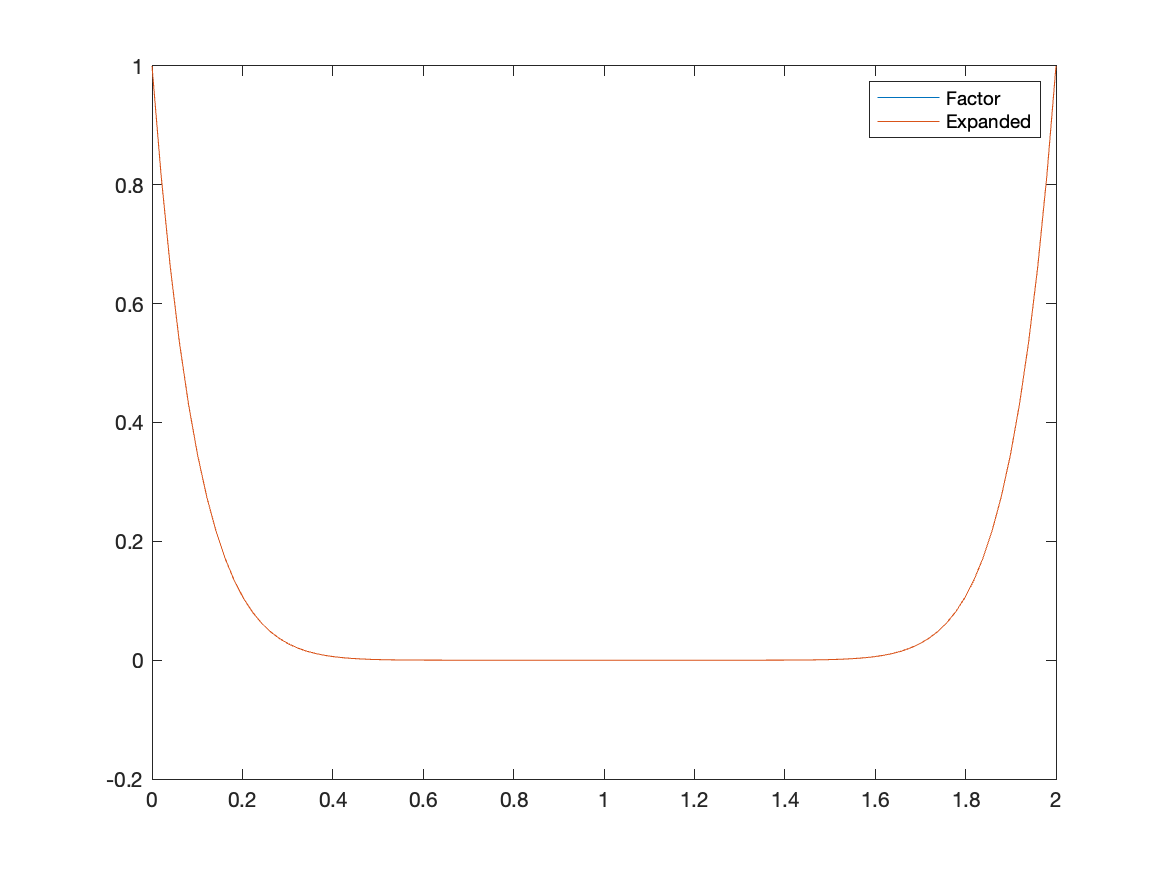
\includegraphics[width=0.48\textwidth]{figs/Ex2_3_1_Ploting_Functions}}
	\hfill
	\subfigure[Zooming In]{\label{zoomingIn}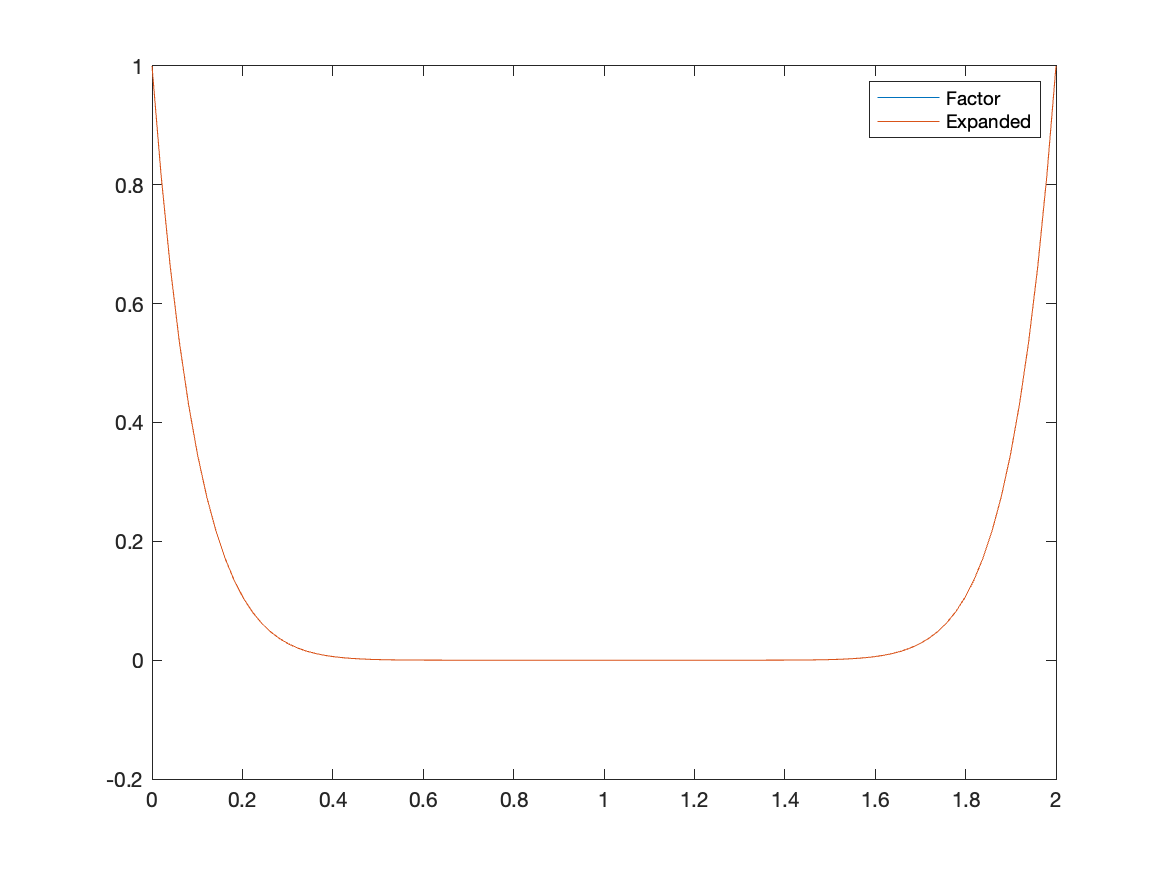
\includegraphics[width=0.5\textwidth]{figs/Ex2_3_1_Ploting_Functions}}\end{figure}
	It seems that the two functions are the same (Fig \ref{plottingFuc}); however if we zooming in (Fig \ref{zoomingIn}), the expanded version introduces more error than the factored version because the expanded version requires more arithmetical operations in it. 
	\end{eg}

\newpage
\section{Solutions of Linear Systems}
\begin{rmk} Assumption throughout this chapter: $\A$ is a square $n\times n$ matrix. \end{rmk}
\subsection{Simply Solved Linear Systems}
\begin{df}{Linear System}
	\begin{itemize}
		\item Equation form: $x_i$ are variables (what we solve for) and $a_{ij}$ are coefficients: \begin{align*}a_{11}x_1+a_{12}x_2+\cdots+a_{1n}x_n&=b_1\\a_{21}x_1+a_{22}x_2+\cdots+a_{2n}x_n&=b_2\\\vdots\\a_{n1}x_1+a_{n2}x_2+\cdots+a_{nn}x_n&=b_n\end{align*} This system has $n$ equations and $n$ variables. 
		\item Matrix form: \[\mqty[a_{11}&a_{12}&\cdots&a_{1n}\\a_{21}&a_{22}&\cdots&a_{2n}\\\vdots&\vdots&\ddots&\vdots\\a_{n1}&a_{n2}&\cdots&a_{nn}]\mqty[x_1\\x_2\\\vdots\\x_n]=\mqty[b_1\\b_2\\\vdots\\b_n]\implies \A x=b,\] where $\A$ is the coefficient matrix, a $n\times n$ matrix, $x$ is the unknown, the solution vector with length $n$, and $b$ is the right hand side, vector with length $n$.
	\end{itemize}	
\end{df}
\begin{thm}{Number of Solutions to a Linear System}
	A linear system $\A x=b$ could have the following numbers of solutions: 
	\begin{itemize}
		\item One unique solution: $\A x=b$ is nonsingular; $\A$ is invertible.
		\item No solutions: $\A x=b$ is singular.
		\item Infinite many solutions: $\A x=b$ is singular. 
	\end{itemize}	
\end{thm}
\begin{thm}{Matrix-Vector Multiplication}
	Let $\A\in\R^{m\times n}$ and $x\in\R^n$. 
	\begin{itemize}
		\item View 1: Row-wise. Let $y=\A x$, then $\dsst y_i=\sum_{j=1}^n a_{ij}x_j$ as the $i^\text{th}$ row of $y$. 
		\item View 2: Column-wise. $\A x$ is a linear combination of columns of $\A$. So, $\dsst y=\sum_{j=1}^nx_j\va{a_j}$, where we regard $\A$ as $\mqty[\va{a_1}&\va{a_2}&\cdots&\va{a_n}]$
	\end{itemize}	
\end{thm}
\begin{lstlisting}[language = Matlab, title = {Row-Wise Vector Multiplication}]
y = zeros(n, 1);
for i = 1:n % loop over rows
	for j = 1:n % loop over sum
		y(i) = y(i) + A(i,j) + x(j);
	end
end
\end{lstlisting}
\begin{lstlisting}[language = Matlab, title = {Row-Wise Vector Multiplication (Vectorization)}]
y = zeros(n, 1);
for i = 1:n % loop over rows
	y(i) = A(i,:) * x(i); % vectorization
end
\end{lstlisting}
\begin{lstlisting}[language = Matlab, title = {Column-Wise Vector Multiplication}]
y = zeros(n, 1);
for j = 1:n % loop over columns
	y = y + x(j) * A(:, j);
end
\end{lstlisting}
\begin{df}{Important Part of a Matrix}
	\begin{itemize}
		\item Diagonal Part
		\item Strictly Upper Triangular Part
		\item Strictly Lower Triangular Part
	\end{itemize}	
\end{df}
\begin{thm}{Solving Diagonal Matrix}
	Given \[\mqty[a_{11}&&\\&\ddots&\\&&a_{nn}]\mqty[x_1\\\vdots\\x_n]=\mqty[b_1\\\vdots\\b_n],\] we have \[a_{11}x_1=b_1;\quad a_{22}x_2=b_2;\quad\cdots\quad a_{nn}x_n=b_n\] So we have \[x_i=\dfrac{b_i}{a_{ii}},\] only if $a_{ii}\neq0.$
	\begin{rmk}$a_{ii}\neq0$ holes if $\A$ is invertible. \end{rmk}
\end{thm}
\begin{rmk}A Diagonal matrix is also a lower triangular matrix or an upper triangular matrix. \end{rmk}
\begin{lstlisting}[language = Matlab, title = {Solving Diagonal Matrix}]
x = zeros(n, 1);
for i = 1:n
	x(i) = b(i) / A(i,i); % overflow and underflow
end
\end{lstlisting}
\begin{thm}{Solving Lower Triangular Systems}
	Given \[\mqty[a_{11}&&&\\a_{21}&a_{22}&&\\\vdots&&\ddots&\\a_{n1}&\cdots&&a_{nn}]\mqty[x_2\\x_2\\\vdots\\x_n]=\mqty[b_1\\b_2\\\vdots\\v_n],\] we have \begin{align*}a_{11}x_1&=b_1\\a_{21}x_1+a_{22}x_{2}&=b_2\\\vdots\\a_{n1}x_1+a_{n2}x_2+\cdots+a_{nn}x_n&=b_n\end{align*} We can use the Forward Substitution to solve: \[x_i=\dfrac{b_1-a_{i1}x_1-a_{i2}x_2-\cdots-a_{i(i-1)}x_{i-1}}{a_{ii}.}\]
\end{thm}
\begin{algorithm}\caption{Row-Oriented Forward Substitution}\SetKwData{And}{\rmfamily{\textbf{and}}}\SetKwData{Or}{\rmfamily{\textbf{or}}}\SetKwData{Break}{\rmfamily{\textbf{break}}}
\KwIn{matrix $\A=\mqty[a_{ij}]$; vector $b=\mqty[b_i]$}
\KwOut{solution vector $x=\mqty[x_i]$}
\BlankLine\Begin{
	\For(\tcp{loop over rows}){i = 1 \KwTo n} { 
		\For(\tcp{loop over columns}) {j = 1 \KwTo i-1} {
			$b_i \coloneqq b_i-a_{ij}x_j$\;
		}
		$x_i \coloneqq b_i/a_{ii}$\;
	}
}
\end{algorithm}
\begin{eg}{}
	Given \[\mqty[-5&&\\3&3&\\2&-5&3]\mqty[x_1\\x_2\\x_3]=\mqty[-10\\3\\21].\] Use column-wise forward substitution to solve this system. 
	\begin{sol}
		In column-wise: \[x_1\mqty[-5\\3\\2]+x_2\mqty[0\\3\\-5]+x_3\mqty[0\\0\\4]=\mqty[-10\\3\\21].\]	
		\begin{enumerate}
			\item Step 1: Solve for $x_1=-10/-5=2.$
			\item Step 2: Plug $x_1=2$ into the equation: \[x_2\mqty[0\\3\\-5]+x_3\mqty[0\\0\\4]=\mqty[-10\\3\\21]-(2)\mqty[-5\\3\\2]=\mqty[0\\-3\\17].\]
			\item Step 3: Solve for $x_2=-3/3=-1$.
			\item Step 4: Plug $x_2=-1$ into the equation: \[x_3\mqty[0\\0\\4]=\mqty[0\\-3\\17]-(-1)\mqty[0\\3\\-5]=\mqty[0\\0\\12].\]
			\item Step 5: Solve for $x_3=12/4=3.$
		\end{enumerate}
	\end{sol}
\end{eg}
\begin{algorithm}\caption{Column-Oriented Forward Substitution}\SetKwData{And}{\rmfamily{\textbf{and}}}\SetKwData{Or}{\rmfamily{\textbf{or}}}\SetKwData{Break}{\rmfamily{\textbf{break}}}
\KwIn{matrix $\A=\mqty[a_{ij}]$; vector $b=\mqty[b_i]$}
\KwOut{solution vector $x=\mqty[x_i]$}
\BlankLine\Begin{
	\For{j = 1 \KwTo n} { 
		$x_j\coloneqq b_j/a_{jj}$\;
		\For{i = j+1 \KwTo n} {
			$b_i \coloneqq b_i-a_{ij}x_j$\;
		}
	}
}
\end{algorithm}
\begin{thm}{Computational Cost of Forward Substitution}
	Number of floating point operations ($+$, $-$, $\times$, $/$) in row $i$ is $1$ division, $(i-1)$ multiplications, and $(i-1)$ subtractions. So, Number of floating points operations, or flops, of the algorithm is \begin{align*}\text{flops}=\sum_{i=1}^n(1+i-1+i-1)&=\sum_{i=1}^n(2i-1)\\&=2\sum_{i=1}^ni-\sum_{i=1}^n1\\&=2\qty[\dfrac{(n+1)(n)}{2}]-n\\&=n^2\end{align*}
	\begin{rmk}It should be the same number of flops if we do column-oriented forward substitution. \end{rmk}
	\begin{rmk} Solving upper triangular system using backward substitution. \end{rmk}
\end{thm}

\subsection{GEPP and Matrix Factorization}
\begin{thm}{Gaussian Elimination}
	In Gaussian Elimination, we are allowed to 
	\begin{enumerate}
		\item Swap rows (exchange, pivot)
		\item Add multiple of one row to another
		\item Multiply row by non-zero scalar. 
	\end{enumerate}
\end{thm}
\begin{rmk}We require the equation with the largest coefficient in magnitude at the top when doing the Gaussian Elimination. This is because we want to divide by large numbers instead of smaller ones (which will cause errors).\end{rmk}
\begin{algorithm}\caption{General Structure of GEPP}\SetKwData{And}{\rmfamily{\textbf{and}}}\SetKwData{Or}{\rmfamily{\textbf{or}}}\SetKwData{Break}{\rmfamily{\textbf{break}}}

\BlankLine\Begin{
	\For{\text{all stages}} { 
		\text{pivot}\;
		\text{eliminate}\;
	}
}
\end{algorithm}
\begin{lstlisting}[language = Matlab, title = {At stage $k$, eliminate $x_k$, from rows $k+1$ to $n$}]
for i = k+1:n
	m(i,k) = a(i,k) / a(k,k); % find the multiplier
	a(i,k) = 0;
	for j = k+1:n
		a(i,j) = a(i,j) - m(i,k) * a(k,j); % could use vectorization
	end
	b(i) = b(i) - m(i,k) * b(k);
end
\end{lstlisting}
\begin{lstlisting}[language = Matlab, title = {Pivoting at stage $k$: find the coefficient with the largest magnitude}]
%% The code tells us which row has the pivot.
p = k;
for i = k+1:n
	if abs(a(p,k)) < abs(a(i,k))
		p = i;
	end
end
%% Swap rows in A and b
A([p,k],:) = A([k,p],:);
b(p) = b(k);
\end{lstlisting}
\begin{thm}{Cost of GEPP}
	At stage $k$, we only focus on rows $k$ through $n$ and columns $k$ through $n$. We have $(n-k)$ divisions for multipliers. For every multiplier we have $(n-k)$ multiplications, which are then used $(n-k)$ times to change each row. So, we have $(n-k)(n-k)$ multiplications in total. Subtractions come with multiplications, so we also have $(n-k)(n-k)$ subtractions. 
\end{thm}
\begin{thm}{Another Perspective on GEPP}
	The process of GEPP can be written as matrix multiplication $\vb E\vb A$, where $\vb E$ is an elementary matrix and act on the rows of $\vb A$.	
\end{thm}
\begin{thm}{Matrix Factorizations: $\vb P\vb A=\vb L\vb U$}
	\[\vb P\vb A=\vb L\vb U,\] where $\vb U$ is upper-triangular, $\vb L$ is lower-triangular, and $\vb P$ is the pivot or permutation matrix.\par 
	This factorization comes from GEPP. Almost all matrices $\vb A$ have $\vb P\vb A=\vb L\vb U$ unless we have a column of all zeros in $\vb A$. \par
\end{thm}
\begin{thm}{Solving $\vb Ax=b$ with $\vb P\vb A=\vb L\vb U$}
	Given $\vb Ax+b$ and pre-computed $\vb P\vb A=\vb L\vb U$: \begin{align*}\vb P\vb A&=\vb Pb\\\vb L\vb U&=\vb Pb\\\vb Ux&=\vb L^{-1}\vb Pb&\text{using forward substitution}\\x&=\vb U^{-1}\vb L^{-1}\vb Pb&\text{using backward substitution}\end{align*}
	This process need around $\bigO\qty(n^2)$ operations. $\bigO(\cdot)$ is the big-O notation, meaning the number is dominated by $n^2$.
\begin{lstlisting}[language=Matlab, title={$\vb P\vb A=\vb L\vb U$ in MATLAB}]
[L, U, P] = lu(A);
% P could be omitted sometimes. 
\end{lstlisting}
\end{thm}
\begin{thm}{Cholesky Factorization}
	If $\A$ is symmetric ($\A=\A^T$) and positive definite (all eigenvalues are positive), then $\A=\vb R^T\vb R$, where $\vb R$ is upper-triangular and $\vb R^T$ is lower-triangular. This factorization is $2$ time less expensive than GEPP. 
\end{thm}
\begin{rmk}
	Choleksy Factorization is just the $\vb P\A=\vb L\vb U$ factorization for SPDs (symmetric positive definite matrices).
\end{rmk}
\begin{thm}{Other Matrix Factorization}
\begin{enumerate}
	\item $\vb Q\vb R$ decomposition: \[\A=\vb Q\vb R,\] where $\vb R$ is upper-triangular and $\vb Q$ is orthogonal such that $\vb Q^T\vb Q=\vb Q^T\vb Q=\vb I$.\par  $\vb Q$ is really easy to be inverted and comes from the Gram-Schmidt process. \par This composition is a bit more expensive than $\vb P\A=\vb L\vb U$.
	\item Singular Value Decomposition (SVD): \[\vb A=\vb U\vb\Sigma\vb V^T,\] where $\vb U$ and $\vb V^T$ are orthogonal and $\vb\Sigma$ is diagonal. This factorization is also more expensive than $\vb P\A=\vb L\vb U$ decomposition.
\end{enumerate}
\end{thm}

\subsection{Measuring Accuracy of Solutions}
\begin{df}{Vector Norms}
	A vector norm is a function $\|\cdot\|:\R^n\to\R$ that satisfies
	\begin{itemize}
		\item \textbf{Positive Definiteness}: $\|x\|\geq0\quad\forall x\in\R^n$ and $\|x\|=0$ if and only if $x=0$.
		\item \textbf{Positive Homogeneity}: $\|cx\|=\qty|c|\|x\|\quad\forall x\in\R^n$ and $c\in\R$.
		\item \textbf{Triangular Inequality}: $\|x+y\|\leq\|x\|+\|y\|\quad\forall x,y\in\R^n$.
	\end{itemize}	
\end{df}
\begin{df}{Common Definitions of Norm}
	\begin{itemize}
		\item Pythagorean Distance: $\|x\|_2=\sqrt{x_1^2+x_2^2+\cdots+x_n^2}$.
		\item Taxicab/Manhattan Distance: $\|x\|_1=\qty|x_1|+\qty|x_2|+\cdots+\qty|x_n|$.
		\item Infinity Norm: $\|x\|_\infty=\dsst\max_{i=1,\dots,n}\qty|x_i|$.
	\end{itemize}	
\end{df}
\begin{prf}
	In this prove, we want to show the $1-$norm is a proper norm.
	\begin{itemize}
		\item \textbf{Positive Definiteness}: Note that $\|x\|_1=\qty|x_1++\cdots+\qty|x_n|\geq0$ since each $\qty|x_j|\geq0$. If one $x_i\neq0$, $\qty|x_i|\geq0$, then $\|x\|_1>0$. So, if $\|x\|_1=0$, it must be $x=0$. $\pqed$
		\item \textbf{Positive Homogeneity}: \begin{align*}\|cx\|_1&=\qty|cx_1|+\qty|cx_2|+\cdots+\qty|cx_n|\\&=\qty|c|\qty|x_1|+\qty|c|\qty|x_2|+\cdots+\qty|c|\qty|x_n|\\&=\qty|c|\qty(\qty|x_1|+\qty|x_2|+\cdots+\qty|x_n|)\\&=\qty|c|\|x\|_1.\pqed\end{align*}
		\item \textbf{Triangle Inequality}: \begin{align*}\|x+y\|_1&=\qty|x_1+y_1|+\qty|x_2+y_2|+\cdots+\qty|x_n+y_n|\\&\leq\qty|x_1|+\qty|y_1|+\qty|x_2|+\qty|y_2|+\cdots+\qty|x_n|+\qty|y_n|\\&=\qty(\qty|x_1|+\qty|x_2|+\cdots+\qty|x_n|)+\qty(\qty|y_1|+\qty|y_2|+\cdots+\qty|y_n|)\\&=\|x\|_1+\|y\|_1.\end{align*}
	\end{itemize}	
\end{prf}
\begin{df}{Matrix Norm}
	A matrix norm is a function $\|\cdot\|:\R^{n\times n}\to\R\st$
	\begin{itemize}
		\item \textbf{Positive Definiteness}: $\|\A\|\geq0$ and $\|\A\|=0$ if and only if $\A=0$.
		\item \textbf{Positive Homogeneity}: $\|c\A\|=\qty|c|\|\A\|$.
		\item \textbf{Triangle Inequality}: $\|\A+\vb{B}\|\leq\|\A\|+\|\vb{B}\|$.
	\end{itemize}	
\end{df}
\begin{df}{Some Matrix Norms}
	\begin{enumerate}
		\item \textbf{Frobenius Norm}: \[\|\A\|_F=\sqrt{\sum_{j=1}^n\sum_{i=1}^na_{ij}^2}.\]
		\item \textbf{Induced Matrix Norm}: Let $\A\in\R^{n\times n}$, $x\in\R^{n\times1}$, and $p=1,2,\infty,\cdots$, then \[\|\A\|_p=\max_{x\neq0}\dfrac{\|\A x\|_p}{\|x\|_p}=\max_{\|x\|_p=1}\|\A x\|_p.\]
	\end{enumerate}	
\end{df}
\begin{rmk}Induced norm intuition: how much does $\|x\|_p$ change when we apply $\A$?\end{rmk}
\begin{thm}{Induced Matrix Norms with different $p$'s}
	\begin{itemize}
		\item $\|\A\|_2=\sigma_1$, the largest singular value. That is, if $\A=\vb U\vb\Sigma\vb V^T$, then $\|\A\|_2$ is the largest entry in $\vb\Sigma$.
		\item $\dsst\|\A\|_1=\max_{j=1,\dots,n}\sum_{i=1}^n\qty|a_{ij}|$, the maximum column sum.
		\item $\dsst\|\A\|_\infty=\max_{i=1,\dots,n}\sum_{j=1}^n\qty|a_{ij}|$, the maximum row sum. 
	\end{itemize}	
\end{thm}
\begin{prf}
	Let's show that $\|\A\|_1$ is the maximum column sum. We will (1) show $\|\A\|_1\leq$ the maximum column sum, and (2) find one case when we attain the upper bound. Given $\|x\|_1=1$, then \begin{align*}\|\A x\|_1=\sum_{i=1}^n\qty|\underbrace{\sum_{j=1}^n a_{ij}x_{j}}_{i-\text{th entry of}\A x}|&\leq\sum_{i=1}^n\sum_{j=1}^n\qty|a_{ij}|\qty|x_j|\\&=\sum_{j=1}^n\qty|x_j|\qty(\sum_{i=1}^n\qty|a_{ij}|)\\&\leq\max_{j=1,\dots,n}\sum_{i=1}^n\qty|a_{ij}|,\text{ when }x\text{ has exactly 1}\text{ entry equal to }1.\end{align*} When $x=e_{j^*}$ be a standard basis vector with $1$ in $j^*$ position, where $j^*$ is the column of $\A$ with maximum column sum, we have \[\|\A e_{j^*}\|_1=\|j-\text{th column of }\A\|_1=\max_{j=1,\dots,n}\sum_{i=1}^n\qty|a_{ij}|.\]	
\end{prf}
\begin{eg}{}
	Given that $\A=\mqty[-1&2\\-12&9]$, find $\|\A\|_1$ and $\|\A\|_\infty$.
	\[\|\A\|_1=\text{maximum column sum}=\max_{j=1,\dots,n}\|\A(:.j)\|_1=13.\]
	\[\|\A\|_\infty=\text{maximum row sum}=21.\]
\end{eg}
\begin{thm}{Submultiplicativity of Induced Norm}
	\[\|\A x\|_p\leq\|\A\|_p\|x\|_p.\]
\end{thm}
\begin{prf}
	By definition, we know $\dsst\|\A\|_p=\max_{x\neq0}\dfrac{\|\A x\|_p}{\|x\|_p}$. Then, \begin{align*}\|\A\|_p&\geq\dfrac{\|\A x\|_p}{\|x\|_p}\\\|\A x\|_p&\leq\|\A\|_p\|x\|_p.\end{align*}	
\end{prf}
\begin{cor}{}
	$\|\A\vb B\|_p\leq\|\A\|_p\|\vb B\|_p.$	
\end{cor}
\begin{df}{Measuring Erros}
	Suppose $x$ is the true solution, and $\hat{x}$ is the approximate solution. Then \begin{align*}\textit{Error}&=\|\hat{x}-x\|\\\textit{Relative Error}&=\dfrac{\|\hat{x}-x\|}{\|x\|},\quad x\neq0.\end{align*}	
	\begin{rmk}In practice, we do not know $x$, the true solution. So this measurement cannot be used.\end{rmk}
\end{df}
\begin{df}{Residual}
	We know $\vb A$, $b$, $\hat{x}$, and we want to solve $\vb Ax=b$. So, the \begin{align*}\textit{Residual}&=\A\hat{x}-b\\\textit{Residual Norm}&=\|\A\hat{x}-b\|\\\textit{Relative Residual Norm}&=\dfrac{\|\A\hat{x}-b\|}{\|b\|}\end{align*}
	
\end{df}
\begin{eg}{}
	Let $\A=\mqty[0.835&0.667\\0.333&0.266], b=\mqty[0.168\\0.067].$ Let $x=\mqty[1\\-1]$ be the exact solution to the system $\A x=b$ and $\hat{x}=\mqty[267\\-334]$, a bad computation of the solution. Then, \begin{align*}\dfrac{\|b-\A\hat{x}\|_2}{\|x\|_2}&\approx0.006\\\dfrac{\|x-\hat{x}\|_2}{\|x\|_2}&\approx\bigO(10^2)\end{align*}	
	\begin{rmk}	The residual norm is not always a good estimate of the relative error.\end{rmk}
\end{eg}
\begin{df}{Ill-Conditioned, Well-Conditioned}
	If the system is linearly dependent, we call the system \textit{ill-conditioned}. If the system is linearly independent, we call it \textit{well-conditioned}.	
\end{df}
\begin{df}{Condition Numbers}
	The condition number of $\A$ is $\kappa\qty(\A)=\|\A\|\|\A^{-1}\|$. Note that $\kappa(\A)\geq1$ and $\kappa(\vb I)=1$. If $\kappa(\A)$ is large, then $\A$ is ill-conditioned. If $\kappa(\A)$ is close to $1$, then $\A$ is well-conditioned. 	
\end{df}
\begin{rmk}
	Some intuition on $\kappa(\A)$: 
	\begin{itemize}
		\item $\|\A\|$: how much $\A$ moves $x$: $\A x=b$.
		\item $\|\A^{-1}\|$: how much $\A^{-1}$ moves $b$: $x=\A^{-1}b$.
	\end{itemize}
	So, if $\kappa(\A)=\|\A\|\|\A^{-1}\|$ is close to $1$, the moves balance each other. If $\kappa(\A)$ is large, then we move the vectors a lot. 
\end{rmk}
\begin{thm}{Upper Bound for Relative Error}
	\[\underbrace{\dfrac{\|x-\hat{x}\|}{\|x\|}}_\text{Relative Error}\leq\kappa(\A)\cdot\underbrace{\dfrac{\|b-\A\hat{x}\|}{\|b\|}}_\text{Relative Residual}=\|\A\|\|\A^{-1}\|\dfrac{\|b-\A\hat{x}\|}{\|b\|}.\]	
\end{thm}
\begin{prf}
	We want to use residual norm to compare $\|x-\hat{x}\|$ and $\|x\|$. Suppose $x$ is the true solution: $b=\A x$. Then, \[\|b\|=\|\A x\|\leq\|\A\|\|x\|.\] So, \begin{equation}\label{eq2}\dfrac{1}{\|x\|}\leq\dfrac{\|\A\|}{\|b\|}\end{equation} Consider the residual: $r=b-\A\hat{x}=\A x-\A\hat{x}=\A\qty(x-\hat{x}).$ So, $x-\hat{x}=\A^{-1}r$. Therefore, \begin{equation}\label{eq3}\|x-\hat{x}\|=\|\A^{-1}r\|\leq\|\A^{-1}\|\|r\|\end{equation} Putting Eq. (\ref{eq2}) and Eq. (\ref{eq3}) together, we have \[\|x-\hat{x}\|\cdot\dfrac{1}{\|x\|}\leq\|\A^{-1}\|\|r\|\cdot\dfrac{\|\A\|}{\|b\|}\] Re-arrange the inequality, we have \[\dfrac{\|x-\hat{x}\|}{\|x\|}\leq\|\A\|\|\A^{-1}\|\dfrac{\|b-\A\hat{x}\|}{\|b\|}.\]
\end{prf}
\begin{rmk}
	Since norms measure how far two things are apart from each other, $\|x-\hat{x}\|=\|\hat{x}-x\|$ and $\|b-\A\hat{x}\|=\|\A\hat{x}-b\|$.
\end{rmk}
\begin{cor}{}
	If $\kappa(\A)\approx1$, then a small residual implies that $\hat{x}$ is a good approximation to the true solution $x$. If $\kappa(\A)$ is large, then we still don't know if $\hat{x}$ is a good approximation to the true solution. 
\end{cor}
\begin{eg}{}
	Given $\A_1=\mqty[1&10\\0&1]$ and $\A_2=\mqty[1&10^6\\0&1]$. Which matrix will have a better approximation to the true solution? 
	\begin{sol}
		\[\kappa_1(\A_1)=\|\A_1\|_1\|\A^{-1}_1\|_1.\] Since $\det(\A_1)=1-0=1,$ we know $\A_1^{-1}=\dfrac{1}{\det(\A_1)}\mqty[1&-10\\0&1]=\mqty[1&-10\\0&1].$ So, \[\kappa_1(\A_1)=\|\A_1\|_1\|\A^{-1}_1\|_1=(11)(11)=121.\] Similarly, \[\kappa_2(\A_2)=\|\A_2\|_1\|\A_2^{-1}\|_1=\qty(1+10^6)\qty(1+10^6)=\bigO(10^12).\] Since $\kappa_2(\A_2)\gg\kappa_1(\A_1)$, $\A_1$ will yield a more accurate approximation.
	\end{sol}
	\begin{rmk}
		Think $\kappa(\A)$ as an indicator for how much movement of $x$ will there be if we apply $\A$ on $x$.	
	\end{rmk}
\end{eg}
\begin{clm}
	Conditioning is inherent to the problem. So, no algorithms can improve conditioning.
\end{clm}
\begin{df}{Algorithm Stability/Backward Stability}
	When we solve $\A x=b$, we will have some algorithm $\hat{x}=\text{algorithm}(\A,b)$. Imagine we run the algorithm in reverse (backwards). We should obtain $\hat{\A}$ and $\hat{b}\st\hat{\A}\hat{x}=\hat{b}$ in exact arithmetic. An algorithm is \textit{backward stable} if $\|\A-\hat{\A}\|$ and $\|b-\hat{b}\|$ are small.	
\end{df}
\begin{rmk}
	Algorithm stability has nothing to do with conditioning.	
\end{rmk}
\begin{eg}{}
	Given $\A=\mqty[\alpha&1\\1&2]$. We know that solving $\A x=b$ using Gaussian Elimination without pivoting, we could get a solution far from true. So, Gaussian Elimination without pivoting is not backward stable. In contrast, GEPP is a backward stable algorithm. 
\end{eg}
\begin{eg}{Is Multiplication Backward Stable?}
	Define \[x\otimes y=\float(\float(x)\times\float(y))\] on a computer with $3$ significant digits. Suppose $x=\dfrac{1}{3}$ and $y=\dfrac{1}{2}$. Then, \[x\otimes y=\float((0.333)(0.500)=0.167;\quad\epsilon_\text{WP}=1.01-1.00=10^{-2}\] Take $\hat{x}=0.334$ and $\hat{y}=0.500$, we get $\hat{x}\hat{y}=0.167$. Since $\|x-\hat{x}\|\approx0.001\leq\dfrac{1}{2}\epsilon_\text{WP}$, we say multiplication is backward stable. Similarly, we could show all floating point operations are backward stable, in fact. 
\end{eg}
\begin{eg}{}
	Prove that $\|\vb Qx\|_2=\|x\|_2$ for any $x\in\R^{n}$ if $\vb Q$ is orthogonal. 
	\begin{prf}
		Since $\vb Q$ is orthogonal, $\vb Q^T\vb Q=\vb Q\vb Q^T=\vb I$. Note that the $2-$norm: \[\|x\|_2^2=x_1^2+x_2^2+\cdots+x_n^2=x^Tx.\] Then, \[\|\vb Qx\|_2^2=\qty(\vb Qx)^T\qty(\vb Qx)=x^T\vb Q^T\vb Qx=x^Tx=\|x\|_2^2.\] So, \[\|\vb Qx\|_2=\|x\|_2.\]
	\end{prf}
	\begin{ext} What is $\|\vb Q\|_2$? What is $\kappa(\vb Q)$?	\end{ext}
	\begin{sol}
		\[\|\vb Q\|_2=\max_{\|x\|_2=1}\dfrac{\|\vb Qx\|_2}{\|x\|_2}=\max_{\|x\|_2=1}\dfrac{\|x\|_2}{\|x\|_2}=\max_{\|x\|_2=1}1=1.\]
		\[\kappa(\vb Q)=\|\vb Q\|_2\|\vb Q^{-1}\|_2=\|\vb Q\|_2\|\vb Q^T\|_2=1\cdot1=1.\]
	\end{sol}
\end{eg}

\newpage
\section{Curve Fitting}
\subsection{Polynomial Interpolation}
\begin{df}{Interpolation}
	A function $p(x)$ interpolates data $\qty{\qty(x_i, f_i)}_{i=0}^N$ if $p(x_i)=f_i$ for $i=0,\dots,N$.
\end{df}
\begin{rmk} Uniqueness of the interpolating polynomial. \end{rmk}
\begin{df}{Polynomial}
	A polynomial $p_k(x)$ is of \textit{degree} $k$ if there are constants $c_0,\dots,c_k\st$\[p_k(x)=c_0+c_1x+\cdots+c_kx^k.\] A polynomial $p_k(x)$ is in \textit{exact degree} $k$ if $c_k\neq0$.
\end{df}
\begin{thm}{Steps for Polynomial Interpolation}
	\begin{enumerate}
		\item Create a problem.
		\begin{itemize}
			\item Find some data.
			\item Design the problem
		\end{itemize}
		\item Choose a degree (based on the number of interpolation points)
		\item Determine the coefficients. $\rightarrow$ Construct a polynomial
		\begin{itemize}
			\item Choose a polynomial basis
			\item Solve a linear system.
		\end{itemize}
		\item Draw the curve: evaluating at lots of points. $\rightarrow$ Evaluate a polynomial
	\end{enumerate}	
\end{thm}
\begin{algorithm}\caption{Constructing a Polynomial Interpolant}
\SetKwData{And}{\rmfamily{\textbf{and}}}\SetKwData{Or}{\rmfamily{\textbf{or}}}\SetKwData{Break}{\rmfamily{\textbf{break}}}
\KwIn{data, $\qty{\qty(x_i, f_i)}_{i=0}^N$; polynomial basis: $\qty{q_j(x)}_{i=0}^N$}
\KwOut{$c_0,\dots,c_M\st\dsst\sum_{j=0}^Mc_jq_j(x_i)=f_i$ for $i=0,\dots,N$}
	Solve for $c_0,\dots,c_M$: \[\begin{cases}c_0q_0(x_0)+c_1q_1(x_0)+\cdots+c_Mq_M(x_0)=f_0\\\vdots\\c_0q_0(x_N)+c_1q_1(x_N)+\cdots+c_Mq_M(x_N)=f_0\end{cases}\] \[\mqty[q_0(x_0)&\cdots&q_M(x_0)\\\vdots&\ddots&\vdots\\q_0(x_N)&\cdots&q_M(x_N)]\mqty[c_1\\\vdots\\c_M]=\mqty[f_0\\\vdots\\f_N]\]
\end{algorithm}
\begin{thm}{Polynomial Uniqueness}
	When the nodes $\qty{\qty(x_i, f_i)}_{i=0}^N$ are distinct, there is a unique polynomial, the interpolating polynomial $p_N(x)$ of degree $N$ that interpolates the data. That is,  \[\mqty[q_0(x_0)&\cdots&q_M(x_0)\\\vdots&\ddots&\vdots\\q_0(x_N)&\cdots&q_M(x_N)]\in\R^{n\times n}\]
\end{thm}
\begin{df}{Power Series}
	\[p_N(x)=c_0+c_1x+c_2x^2+\cdots+c_Nx^N\]
	The Vandermonde Matrix is defined as \[\mqty[1&x_0&\cdots&x_0^N\\\vdots&\vdots&\ddots&\vdots\\1&x_N&\cdots&x_N^N].\]
	\begin{itemize}
		\item Pros: easy to understand and implement
		\item Cons: ill-conditioning, near singularity of the Vandermonde matrix, when $\qty|x_i-x_j|$ is small. 
	\end{itemize}
\end{df}
\begin{eg}{Power Series}
	Interpolate the points $\qty{(-1,0), (0,1), (1,3)}$.
	\begin{sol}
		Suppose $p_2(x)=c_0+c_1x+c_2x^2$. Then, \begin{align*}(-1,0):\ p_2(-1)&=c_0+c_1(-1)+c_2(-1)^2=0\\(0,1):\ p_2(0)&=c_0+c_1(0)+c_2(0^2)=1\\(1,3):\ p_2(1)&=c_0+c_1(1)+c_2(1)^2=3.\end{align*} In matrix form: \[\mqty[1&-1&1\\1&0&0\\1&1&1]\mqty[c_0\\c_1\\c_2]=\mqty[0\\1\\3]\implies\mqty[c_0\\c_1\\c_2]=\mqty[1\\3/2\\1/2].\]
	\end{sol}
\end{eg}
\begin{df}{Newton Form}
	\[p_N(x)=b_0+b_1\qty(x-x_0)+b_2(x-x_0)(x-x_1)+\cdots+b_N(x-x_0)(x-x_1)\cdots(x-x_{N-1}).\]
	\begin{itemize}
		\item Pros: we are having a lower triangular system: 
		\begin{align*}p_N(x_0)&=b_0\\p_N(x_1)&=b_0+b_1(x-x_0)\\p_N(x_2)&=b_0+b_1(x-x_0)+b_2(x-x_0)(x-x_1).\end{align*}
	\end{itemize}
\end{df}
\begin{eg}{Newton Form}
	Interpolate the points $\qty{(-1,0), (0,1), (1,3)}$.
	\begin{sol}
		\begin{align*}p_N(x)&=b_0+b_1(x-(-1))+b_2(x-(-1))(x-0)\\p_N(-1)&=b_0\\p_N(0)&=b_0+b_1\\p_N(1)&=b_1+2b_1+2b_2\end{align*} In matrix form: \[\mqty[1&0&0\\1&1&0\\1&2&2]\mqty[b_0\\b_1\\b_2]=\mqty[0\\1\\3]\xrightarrow[\text{Substitution}]{\text{Forward}}\mqty[b_0\\b_1\\b_2]=\mqty[0\\1\\1/2].\]
	\end{sol}
\end{eg}
\begin{df}{Lagrange Polynomials}
	\begin{itemize}
		\item Coefficient $=$ function values $f_i$. $\Longrightarrow$ we don't need to solve anything
		\item \[\l(x):\begin{cases}1\quad\text{at }x=x_i\\0\quad\text{ at}x=x_j,\ j\neq i\end{cases}\] Now, we want to construct a polynomial that has roots at all the nodes: \[\omega(x)=(x-x_0)(x-x_1)\cdots(x-x_N).\] Then, if we assume we have distinct noes, we have \[\l_0(x)=\dfrac{(x-x_1)(x-x_2)\cdots(x-x_N)}{(x_0-x_1)(x_0-x_2)\cdots(x_0-x_N)}\] \[\l_3(x)=\dfrac{(x-x_0)(x-x_1)(x-x_2)(x-x_4)\cdots(x-x_N)}{(x_3-x_0)(x_3-x_1)(x_3-x_2)(x_3-x_4)\cdots(x_3-x_N)}\] Generalizing, we have \[\l_k(x)=\dfrac{(x-x_0)(x-x_1)\cdots(x-x_{k-1})(x-x_{k+1})\cdots(x-x_N)}{\text{numerator evaluated at }x=x_k}=\prod_{j=0,\ j\neq k}^N=\dfrac{x-x_j}{x_k-x_j}.\]
		\item $\dsst p_N(x)=\sum_{i=0}^N f_i\cdot\l_i(x)$.
		\item Pros: No solving. Great for theory.
		\item Cons: constructing $\l_i(x)$ is tricky.
	\end{itemize}
\end{df}
\begin{eg}{Lagrange Polynomials}
	Interpolate the points $\qty{(-1,0), (0,1), (1,3)}$.	
	\begin{sol}
		\[\l_0(x)=\dfrac{(x-0)(x-1)}{(-1-0)(-1-1)};\quad\l_1(x)=\dfrac{(x-(-1))(x-1)}{(0-(-1))(0-1)};\quad\l_2(x)=\dfrac{(x-(-1))(x-0)}{(1-(-1))(1-0)}\] So, \[p_N(x)=f_0\l_0(x)+f_1\l_1(x)+f_2\l_2(x).\]
	\end{sol}
\end{eg}
\begin{df}{Chebyshev Polynomial}
	\begin{itemize}
		\item Only works for domain $[-1,1]$, but easy to extend to $[a,b]$.
		\item $T_j(x)=\cos(j\cdot\arccos(x)),\quad j=0,\dots,N$. Therefore, $T_0(x)=\cos(0\cdot\arccos(x))=1$ and $T_1=\cos(1\cdot\arccos(x))=x.$ By trigonometric identities, we can show \[T_{j+1}=2xT_j(x)-T_{j-1}(x).\]
		\begin{rmk}Domain is limited to $[-1,1]$ because $\arccos(x)$ can only take $x\in[-1,1].$\end{rmk}
		\item We solve for $d_0,\dots,d_N$, where \[p_N(x)=d_0T_0(x)+d_1T_1(x)+d_2T_2(x)+\cdots+d_NT_N(x)\]
		\item Pros: Nice numerical properties due to oscillation.
		\item Cons: Highly non-intuitive. 
	\end{itemize}
\end{df}
\begin{eg}{Chebyshev Polynomial}
	Interpolate the points $\qty{(-1,0), (0,1), (1,3)}$.	
	\begin{sol}
		Assume $p_2(x)=d_0T_0+d_1T_1(x)+d_2T_2(x)$, where $T_0(x)=1$, $T_1(x)=x$, $T_2(x)=2x^2-1$. Then, \begin{align*}p_2(-1)&=d_0+d_1(-1)+d_2(1)\\p_2(0)&=d_0+d_1(0)+d_2(-1)\\p_2(1)&=d_0+d_!(1)+d_2(1)\end{align*} In matrix form, we have \[\mqty[1&-1&1\\1&0&-1\\1&1&1]\mqty[d_0\\d_1\\d_2]=\mqty[0\\1\\3]\implies\mqty[d_0\\d_1\\d_2]=\mqty[5/4\\3/2\\1/4]\]
	\end{sol}
\end{eg}

\subsection{Error in Polynomial Interpolation}
\begin{rmk} Set-up:
	\begin{itemize}
		\item $f(x)$, the unknown function
		\item $\qty{(x_i,f_i)}_{i=0}^N$, data, where $f_i=f(x_i)$.
		\item $p_N(x)$, degree $N$ interpolant
		\item Our goal is to find $\mathrm{error}=f(x)-p_N(x)$. Note that at $x=x_i$, $f(x_i)-p_N(x_i)=0$ for $i=1,\dots,N$. So, $x_i$ are roots of $f(x_i)-p_N(x_i)$. Recall that $x_i$ are also roots of $\omega(x)=(x-x_0)(x-x_1)\cdots(x-x_N)$. We wonder if we can build a connection between them.
	\end{itemize}	
\end{rmk}
\begin{thm}{}
	$\exists\ \xi_x$, a point on $[a,b]$ depends on $x$ such that \[f(x)-p_N(x)=\dfrac{\omega(x)}{(N+1)!}f^{(N+1)}(\xi_x).\]
\end{thm}
\begin{eg}{}
	Suppose $f(x)=x^2$ on $[0,1]$. We have data $\qty{(0,0), (1,1)}$ and interpolant $p_1(x)=x$.\par  Then, \[f(x)-p_1(x)=x^2-x\] and \[\omega(x)=(x-0)(x-1)=x^2-x.\]\par Therefore, \[\text{LHS}=\dfrac{\omega(x)}{(N+1)!}f^{(N+1)}(\xi_x)=\dfrac{x^2-x}{(1+1)!}f''(\xi_x)=\dfrac{x^2-x}{2!}(2)=x^2-x=\text{RHS}\]
\end{eg}
\begin{eg}{}
	Suppose $f(x)=x^3$ on $[0,1]$. We have data $\qty{(0,0), (1,1)}$ and interpolant $p_1(x)=x$.\par Then, \[f(x)-p_1(x)=x^3-x\] and \[\omega(x)=(x-0)(x-1)=x^2-x.\]\par Therefore, \[\text{RHS}=\dfrac{\omega(x)}{(N+1)!}f^{(N+1)}(\xi_x)=\dfrac{x^2-x}{(1+1)!}f''(\xi_x)=\dfrac{x^2-x}{2}(6\xi_x)=x^2-x.\]\par Question: Can we find a $\xi_x$ where $\dfrac{x^2-x}{2}(6\xi_x)=x^2-x$.\par Answer: Say we want to evaluate error at $x=\dfrac{1}{2}$, we can certainly find some $\xi_x=\xi_\frac{1}{2}$ such that \[\qty(\dfrac{1}{2})^2-\qty(\dfrac{1}{2})=\dfrac{(1/2)^2-(1/2)}{2}(6\xi_x).\]
\end{eg}
\begin{rmk}
	Some intuition on why this equation holds. 
	\begin{itemize}
		\item When is $f(x)-p_N(x)=0$? At $x_0,\dots,x_N$ due to interpolation.
		\item When is $\omega(x)=0$? At $x_0,\dots,x_N$ due to construction.
		\item So, $f(x)-p_N(x)$ has roots $x_0,\dots,x_N$, which means we can ``factor'' out the roost using $\omega(x)$: $f(x)-p_N(x)=\omega(x)g(x)$.
		\item What is $\xi_x$? It is found through the Rolle's Theorem. a special case for the Mean Value Theorem: If $f(a)=f(b)=0$, then $\exists\xi\in[a,b]\st f'(\xi)=0$.
	\end{itemize}
\end{rmk}
\begin{thm}{Make Error Small}
	\[\max_{x\in[a,b]}\qty|f(x)-p_N(x)|\leq\underbrace{\max_{x\in[a,b]}\qty|\omega(x)|}_\text{make this small!}\cdot\dfrac{\overbrace{\max_{z\in[a,b]}\qty|f^{(N+1)}(z)|}^\text{typically unknown}}{(N+1)!}\]	
\end{thm}
\begin{thm}{Make $\qty|\omega(x)|$ small}
	\[\omega(x)=(x-x_0)(x-x_1)\cdots(x-x_N)\] Choose $x_i$ so that usually $x$ is ``close'' to some $x_i$: Chebyshev points, roots of Chebyshev polynomials: \[x_i=\cos\qty(\dfrac{2i-1}{2n}\pi),\quad i=1,\dots,n\]
\end{thm}
\begin{thm}{}
	\[\qty|\omega(x)|\leq\qty|b-a|^{N+1}\]
	\begin{rmk}This inequality is true because $\omega(x)$ can be regarded as distances from $x$ to $x_i$'s. Hence, another approach to make $\qty|\omega(x)|$ smaller is to make the interval $[a,b]$ smaller. \end{rmk}
\end{thm}
\begin{df}{Linear Splines}
	\begin{itemize}
		\item Data: $\qty{(x_i,f_i)}_{i=1}^N$
		\item Ordering: $a=x_0<x_1<x_2<\cdots<x_N=b$
		\begin{rmk} We do not require equally spaced points here. \end{rmk}
		\item Linear Splines: \[S_{1,N}(x)=\begin{cases}f_0\cdot\dfrac{x-x_1}{x_0-x_1}+f_1\cdot\dfrac{x-x_0}{x_1-x_0},&\quad x\in[x_0,x_1]\\f_1\cdot\dfrac{x-x_2}{x_1-x_2}+f_2\cdot\dfrac{x-x_1}{x_2-x_1},&\quad x\in[x_1,x_2]\\\vdots\\f_{N-1}\cdot\dfrac{x-x_N}{x_{N-1}-x_N}+f_N\cdot\dfrac{x-x_{N-1}}{x_N-x_{N-1}},&\quad x\in[x_{N-1},x_N]\end{cases},\] where $1$ indicates the degree of each piece ($1$ for linear) and $N$ is the number of intervals ($N+1$ points create $N$ intervals)
	\end{itemize}	
\end{df}
\begin{eg}{}
	Given $\qty{(-1,0),(0,1),(1,3)}$. Construct $S_{1,2}(x)$.
	\begin{sol}
		\[S_{1,2}=\begin{cases}0\cdot\dfrac{x-0}{(-1)-0}+1\cdot\dfrac{x-(-1)}{0-(-1)}=x+1&\quad x\in[-1,0]\\1\cdot\dfrac{x-1}{0-1}+3\cdot\dfrac{x-0}{1-0}=1-x+3x=2x+1&\quad x\in[0,1]\end{cases}.\]
	\end{sol}
\end{eg}
\begin{df}{Linear B-Splines}
	We define the linear B-splines basis as follows: \[L_0(x)=\begin{cases}\dfrac{x-x_1}{x_0-x_1}&\quad x\in[x_0,x_1]\\0&\quad o/w\text{ (otherwise)}\end{cases}\] \[L_i(x)=\begin{cases}\dfrac{x-x_{i-1}}{x_i-x_{i-1}}&\quad x\in[x_{i-1},x_i]\text{ (left of }x_i)\\\dfrac{x-x_{i+1}}{x_i-x_{i+1}}&\quad x\in[x_i,x_{i+1}]\text{ (right of }x_i)\\0,&\quad o/w\end{cases},\quad i=1,\dots,N-1.\] \[L_N(x)=\begin{cases}\dfrac{x-x_{N-1}}{x_{N}-x_{N-1}}&\quad x\in[x_{N-1},x_N]\\0&\quad o/w\end{cases}\] Therefore, we can write the linear splines as \[S_{1,N}(x)=f_0L_0(x)+f_1L_1(x)+\cdots+f_NL_N(x).\]
\end{df}
\begin{df}{Cubic Splines}
	\[S_{3,N}(x)=\begin{cases}p_1(x)=a_{1,0}+a_{1,1}x+a_{1,2}x^2+a_{1,3}x^3&\quad x\in[x_0,x_1]\\p_2(x)=a_{2,0}+a_{2,1}x+a_{2,2}x^2+a_{2,3}x^3&\quad x\in[x_1,x_2]\\\vdots\\p_N(x)=a_{N,0}+a_{N,1}x+a_{N,2}x^2+a_{N,3}x^3&\quad x\in[x_{N-1},x_N]\end{cases},\] where $a_{i,j}$ are unknowns. We have in total $4N$ unknowns, so we need $4N$ equations to solve them. We want the splines to interpolate and continuous. So, for $i=1,\dots, N$ we have \[p_i(x_{i-1})=f_{i-1}\quad\text{and}\quad p_i(x_i)=f_i,\] which gives us in total $2N$ equations. To ensure continuous, we want the derivatives to be continuous, so we have \[p'_i(x_i)=p'_{i+1}(x_i)\quad\text{for }i=1,\dots,N-1,\] which gives us another $N-1$ equations. To further ensure continuous and smoothy, we need continuous second derivatives, so we have \[p_i''(x_i)=p_{i+1}''(x_i)\quad\text{for }i=1,\dots,N-1,\] which also gives us $N-1$ equations. Now, we have in total $4N-2$ equations, and we cannot take the $3^\text{rd}$ derivatives because after taking the $3^\text{rd}$ derivatives, there will be only constants left. Hence, we still need $2$ more equations, and there are several different approaches: 
	\begin{itemize}
		\item Natural boundary conditions: \[p_1''(x_0)=0;\qquad p''_N(x_N)=0.\]
		\item Second derivative conditions: \[p_1''(x_0)=f''(x_0);\qquad p_N''(x_N)=f''(x_N)\] This condition is not always helpful because we don't always know the information on the original function.
		\item First derivative conditions: \[p_1'(x_0)=f'(x_0);\qquad p_N'(x_N)=f'(x_N).\]
		\item Not-a-knot condition: \[p_1'''(x_1)=p_2'''(x_1);\qquad p_{N-1}'''(x_{N-1})=p_N'''(x_{N-1})\]
	\end{itemize}
\end{df}
\begin{df}{Cubic B-Splines}
	Assume we have equally spaced points $x_0$, $x_1=x_0+h$, $x_2=x_1+h,\cdots$. We want to find $B_p(x)$ center at $x_p$: 
	\begin{center}
	\tikzset{every picture/.style={line width=0.75pt}} 
	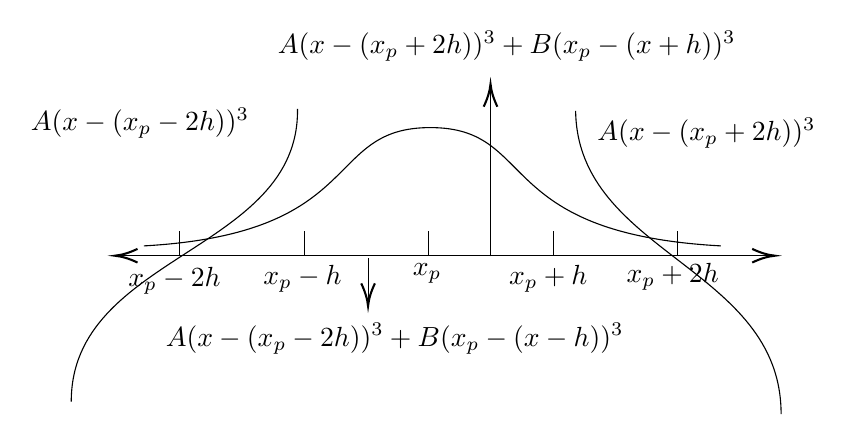
\begin{tikzpicture}[x=0.75pt,y=0.75pt,yscale=-1,xscale=1]
	\draw    (100.73,211) -- (414.73,211) ;
	\draw [shift={(416.73,211)}, rotate = 180] [color={rgb, 255:red, 0; green, 0; blue, 0 }  ][line width=0.75]    (10.93,-3.29) .. controls (6.95,-1.4) and (3.31,-0.3) .. (0,0) .. controls (3.31,0.3) and (6.95,1.4) .. (10.93,3.29)   ;
	\draw [shift={(98.73,211)}, rotate = 0] [color={rgb, 255:red, 0; green, 0; blue, 0 }  ][line width=0.75]    (10.93,-3.29) .. controls (6.95,-1.4) and (3.31,-0.3) .. (0,0) .. controls (3.31,0.3) and (6.95,1.4) .. (10.93,3.29)   ;
	\draw    (250,199.27) -- (250,211) ;
	\draw    (310,199.27) -- (310,211) ;
	\draw    (370,199.27) -- (370,211) ;
	\draw    (190,199.27) -- (190,211) ;
	\draw    (130,199.27) -- (130,211) ;
	\draw    (77.73,281.27) .. controls (77.73,210.27) and (187.73,209.27) .. (186.73,140.27) ;
	\draw    (419.73,287.27) .. controls (419.73,216.27) and (321.73,210.27) .. (320.73,141.27) ;
	\draw    (112.73,206.27) .. controls (220.73,200.27) and (198.73,149.27) .. (250.73,149.27) .. controls (302.73,149.27) and (279.73,200.27) .. (390.73,206.27) ;
	\draw    (220.73,212.27) -- (220.73,233.27) ;
	\draw [shift={(220.73,235.27)}, rotate = 270] [color={rgb, 255:red, 0; green, 0; blue, 0 }  ][line width=0.75]    (10.93,-3.29) .. controls (6.95,-1.4) and (3.31,-0.3) .. (0,0) .. controls (3.31,0.3) and (6.95,1.4) .. (10.93,3.29)   ;
	\draw    (279.73,211.27) -- (279.73,130.27) ;
	\draw [shift={(279.73,128.27)}, rotate = 90] [color={rgb, 255:red, 0; green, 0; blue, 0 }  ][line width=0.75]    (10.93,-3.29) .. controls (6.95,-1.4) and (3.31,-0.3) .. (0,0) .. controls (3.31,0.3) and (6.95,1.4) .. (10.93,3.29)   ;
	\draw (241,213.4) node [anchor=north west][inner sep=0.75pt]    {$x_{p}$};
	\draw (287.37,214.4) node [anchor=north west][inner sep=0.75pt]    {$x_{p} +h$};
	\draw (344,213.4) node [anchor=north west][inner sep=0.75pt]    {$x_{p} +2h$};
	\draw (169,214.4) node [anchor=north west][inner sep=0.75pt]    {$x_{p} -h$};
	\draw (104,215.4) node [anchor=north west][inner sep=0.75pt]    {$x_{p} -2h$};
	\draw (57,138.4) node [anchor=north west][inner sep=0.75pt]    {$A( x-( x_{p} -2h))^{3}$};
	\draw (330,143.4) node [anchor=north west][inner sep=0.75pt]    {$A( x-( x_{p} +2h))^{3}$};
	\draw (122,242.4) node [anchor=north west][inner sep=0.75pt]    {$A( x-( x_{p} -2h))^{3}+B( x_p-( x-h))^{3}$};
	\draw (176,101.4) node [anchor=north west][inner sep=0.75pt]    {$A( x-( x_{p} +2h))^{3}+B( x_p-( x+h))^{3}$};
	\end{tikzpicture}
	\end{center}
	We require $B_p(x_p)=1$, so we have \[A\qty(x-\qty(x_p-2h))^3+B\qty(x-\qty(x_p-h))^3=1.\] We require continuity, so \[A( x-( x_{p} -2h))^{3} B( x-( x-h))^{3}=A( x-( x_{p} +2h))^{3} B( x-( x+h))^{3}.\] Solving the system, we will have \[B_p(x)=\begin{cases}0&\quad x<x_p-2h\\\dfrac{1}{4h^3}\qty(x-\qty(x_p-2h))^3&\quad x_p-2h\le x<x_p-h\\\dfrac{1}{4h^3}\qty(x-(x_p-2h))^3-\dfrac{1}{h^3}\qty(x-(x_p-h))^3&\quad x_p-h\le x<x_p\\-\dfrac{1}{4h^3}\qty(x-(x_p+2h))^3+\dfrac{1}{h^3}\qty(x-(x_p+h))^3&\quad x_p\le x<x_p+h\\-\dfrac{1}{4h^3}\qty(x-(x_p+2h))^3&\quad x_p+h\le x+x_p+2h\\0&\quad x_p+2h\le x\end{cases}\] Then, we have \[S_N(x)=\sum_{i=-1}^{N+1}a_i\cdot B_i(x),\] where \[B_p\qty(x_{p-1})=\dfrac{1}{4};\quad B_p(x_p)=1;\quad B_p\qty(x_{p+1})=\dfrac{1}{4}\]
\end{df}

\subsection{Least Square}
\begin{df}{Least Square Polynomial}
	Let $q_M(x)$ be a polynomial of degree $M$. We want to measure the error between $q_M(x)$ and $f(x)$ with data $\qty{(x_i,f_i)}_{i=0}^N$. We define \[\sigma\qty(q_M(x))\equiv\sum_{r=0}^N\qty{q_M(x_r)-f_r}^2\] The \textit{least square polynomial} of degree $M$, $p_M(x)$, satisfies \[\sigma\qty(p_M)\le\sigma(q_M)\] for any other degree $M$ polynomial $q_M(x)$.
\end{df}
\begin{eg}{Find the Best Fit Line}
	\begin{center}\begin{tabular}{c|c|c}
		$i$&$x_i$&$f_i$\\\hline
		$0$&$1$&$2$\\
		$1$&$3$&$4$\\
		$2$&$4$&$3$\\
		$3$&$5$&$1$
	\end{tabular}\end{center}
	\begin{sol}
		Suppose $p_1(x)=a_0+a_1x$. Then, \[\sigma\qty(p_1)=\sum_{r=0}^3\qty{a_0+a_1x_r-f_r}^2\] To minimize $\sigma(p_1)$, we set $\dsst\pdv{\sigma}{a_0}=\pdv{\sigma}{a_0}=0$: \begin{align*}\pdv{\sigma\qty(p_1)}{a_0}&=\sum_{r=0}^32\qty(a_0+a_1x_r-f_r)=0\\\pdv{\sigma\qty(p_1)}{a_0}&=\sum_{r=0}^22x_r\qty(a_0+a_1x_r-f_r)=0\end{align*} Plugging in data, we have \[\pdv{\sigma\qty(p_1)}{a_0}=2(4a_0+13a_1-10)=0;\quad \pdv{\sigma\qty(p_1)}{a_0}=2(13a_0+51a_1-31)=0\] Solve the following system: \[\mqty[4&13\\13&51]\mqty[a_0\\a_1]=\mqty[10\\31]\implies\mqty[a_0\\a_1]=\mqty[107/35\\-6/35].\]
	\end{sol}
\end{eg}
\begin{df}{Best Fit Polynomial}
	\[q_M(x)=a_0\phi_o(x)+a_1\phi_1(x)+\cdots+a_M\phi_M(x).\] We want $q_M(x)$ to fit data $\qty{(x_i,f_i)}_{i=0}^N$ as best as we can, so we compute the error \[\sigma(q_M)=\sum_{r=0}^N\qty{q_M(x_r)-f_r}^2=\sum_{r=0}^N\qty{a_0\phi_o(x_r)+a_1\phi_1(x_r)+\cdots+a_M\phi_M(x_r)-f_r}^2.\] In matrix form (vector 2-norm), we have \[\sigma(q_M)=\|\vb Va-f\|_2^2.\] That is, \[\sigma(q_M)=\Bigg\|\mqty[\phi_0(x_0)&\phi_1(x_0)&\cdots&\phi_M(x_0)\\\phi_0(x_1)&\phi_1(x_1)&\cdots&\phi_M(x_1)\\\vdots&\vdots&\ddots&\vdots\\\phi_0(x_N)&\phi_1(x_N)&\cdots&\phi_M(x_N)]\mqty[a_0\\\vdots\\a_M]-\mqty[f_0\\f_1\\\vdots\\f_N]\Bigg\|_2^2\] To find a $p_M$ minimizes $\|\vb Va-f\|_2^2$, we solve the normal equations, that is \[\vb V^T\vb Va=\vb V^Tf.\] Solving the normal equation is equivalent to solving the least square problems.
\end{df}
\begin{eg}{Basis}
	For $\phi_i(x)=x^j$, the power series, the big matrix $\vb V$ becomes \[\mqty[1&x_0&x_0^2&\cdots&x_0^M\\1&x_1&x_1^2&\cdots&x_1^M\\\vdots&\vdots&\vdots&\ddots&\vdots\\ 1&x_N&x_N^2&\cdots&x_N^M]\]	This is consistent with the Vandermonde matrix. The matrix might not necessarily be a squared matrix. 
\end{eg}
\begin{eg}{Solving the Normal Equation}
	Find the best fit equation $p_2(x)=a_1+a_1x+a_2x^2$.
	\begin{center}\begin{tabular}{c|c|c}$i$&$x_i$&$f_i$\\\hline$0$&$-2$&$6$\\$1$&$-1$&$3$\\$2$&$0$&$1$\\$3$&$1$&$3$\\$4$&$2$&$6$\end{tabular}\end{center}
	\begin{sol}
		Construct $\vb V$ (power series): \[\vb V=\mqty[1&-2&4\\1&-1&1\\1&0&0\\1&1&1\\1&2&4];\qquad f=\mqty[6\\3\\1\\3\\6]\]	 Construct $\vb V^T\vb V$ and $\vb V^Tf$: \[\vb V^T\vb V=\mqty[5&0&0\\0&10&-18\\10&-18&34];\qquad\vb V^Tf=\mqty[19\\0\\54]\]
		\begin{rmk} In most cases of this class, $\vb V^T\vb V$ will be symmetric, positive, definite (having positive eigenvalues), so $\vb V^T\vb V$ is invertible\end{rmk}
		Solve $\vb V^T\vb Va=\vb V^Tf$: \verb| MATLAB: (V'*V)\(V'*f); % worse conditioning| \[a\approx\mqty[1.5143\\0\\1.1429].\]
	\end{sol}
\end{eg}
\begin{rmk}
	Important Points.
	\begin{itemize}
		\item $\vb V$ is an $(N+1)\times(M+1)$ matrix, and $M<N$.
		\item If $M<N$ and $x_i$ are distinct, $\vb V^T\vb V$ will be SPD, and $p_M$ is unique. 
		\item If $M=N$, we are back to polynomial interpolation.
		\item In practice, least square polynomial is more useful than interpolation for data analysis.
	\end{itemize}	
\end{rmk}
\begin{rmk}
	Why does the normal equation work?  - Linear Algebra. 
	\begin{center}
	\tikzset{every picture/.style={line width=0.75pt}}
	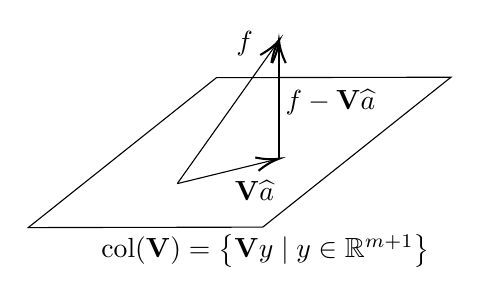
\begin{tikzpicture}[x=0.75pt,y=0.75pt,yscale=-1,xscale=1]
	\draw   (189.7,188.22) -- (302.7,188) -- (212.02,260.23) -- (99.02,260.45) -- cycle ;
	\draw    (170.82,239.27) -- (217.88,227.75) ;
	\draw [shift={(219.82,227.27)}, rotate = 166.24] [color={rgb, 255:red, 0; green, 0; blue, 0 }  ][line width=0.75]    (10.93,-3.29) .. controls (6.95,-1.4) and (3.31,-0.3) .. (0,0) .. controls (3.31,0.3) and (6.95,1.4) .. (10.93,3.29)   ;
	\draw    (170.82,239.27) -- (218.66,171.9) ;
	\draw [shift={(219.82,170.27)}, rotate = 125.38] [color={rgb, 255:red, 0; green, 0; blue, 0 }  ][line width=0.75]    (10.93,-3.29) .. controls (6.95,-1.4) and (3.31,-0.3) .. (0,0) .. controls (3.31,0.3) and (6.95,1.4) .. (10.93,3.29)   ;
	\draw    (219.82,227.27) -- (219.82,172.27) ;
	\draw [shift={(219.82,170.27)}, rotate = 90] [color={rgb, 255:red, 0; green, 0; blue, 0 }  ][line width=0.75]    (10.93,-3.29) .. controls (6.95,-1.4) and (3.31,-0.3) .. (0,0) .. controls (3.31,0.3) and (6.95,1.4) .. (10.93,3.29)   ;
	\draw (198,164.4) node [anchor=north west][inner sep=0.75pt]    {$f$};
	\draw (221.82,192.67) node [anchor=north west][inner sep=0.75pt]    {$f-\mathbf{V}\hat{a}$};
	\draw (197.32,236.67) node [anchor=north west][inner sep=0.75pt]    {$\mathbf{V}\hat{a}$};
	\draw (133,262.4) node [anchor=north west][inner sep=0.75pt]    {$\mathrm{col}(\mathbf{V}) =\left\{\mathbf{V} y\mid y\in \mathbb{R}^{m+1}\right\}$};
	\end{tikzpicture}
	\end{center}
	Our goal: $\dsst\min_{a}\|\vb Va-f\|_2^2$. We want a nontrivial $\hat{a}$ such that \begin{align*}\qty(\vb V\hat{a})^T-\qty(f-\vb V\hat{a})&=0\\\hat{a}^T\qty(\vb V^T\qty(f-\vb V\hat{a}))&=0\\\vb V^Tf-\vb V^T\vb V\hat{a}&=0&normal\ equation\end{align*}
\end{rmk}
\begin{df}{Solving Least Squares with Matrix Factorization}
	We will use $\vb Q\vb R$ factorization. 
	\begin{itemize}
		\item $\vb V=\vb Q\vb R$, where $\vb Q$ is orthogonal and $\vb R$ is upper triangular. 
		\begin{center}
		\tikzset{every picture/.style={line width=0.75pt}} 
		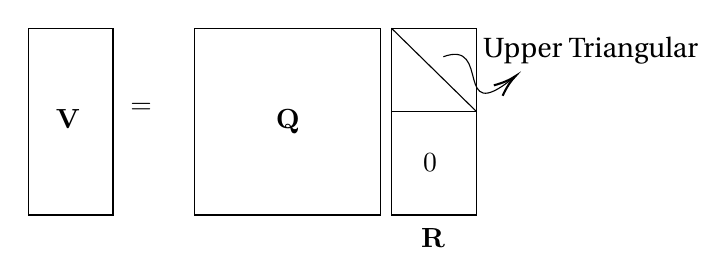
\begin{tikzpicture}[x=0.75pt,y=0.75pt,yscale=-1,xscale=1]
		\draw   (100,120.27) -- (140.82,120.27) -- (140.82,210.27) -- (100,210.27) -- cycle ;
		\draw   (180,120.27) -- (269.82,120.27) -- (269.82,210.27) -- (180,210.27) -- cycle ;
		\draw   (275,120.27) -- (315.82,120.27) -- (315.82,210.27) -- (275,210.27) -- cycle ;
		\draw   (275,120.27) -- (315.82,120.27) -- (315.82,160.27) -- (275,160.27) -- cycle ;
		\draw    (275,120.27) -- (315.82,160.27) ;
		\draw    (300,134) .. controls (323.47,125.4) and (304.41,167.96) .. (333.46,144.4) ;
		\draw [shift={(334.82,143.27)}, rotate = 140.01] [color={rgb, 255:red, 0; green, 0; blue, 0 }  ][line width=0.75]    (10.93,-3.29) .. controls (6.95,-1.4) and (3.31,-0.3) .. (0,0) .. controls (3.31,0.3) and (6.95,1.4) .. (10.93,3.29)   ;
		\draw (112,158.4) node [anchor=north west][inner sep=0.75pt]    {$\mathbf{V}$};
		\draw (218,158.4) node [anchor=north west][inner sep=0.75pt]    {$\mathbf{Q}$};
		\draw (288,215.4) node [anchor=north west][inner sep=0.75pt]    {$\mathbf{R}$};
		\draw (317.82,123.27) node [anchor=north west][inner sep=0.75pt]   [align=left] {Upper Triangular};
		\draw (289,179.4) node [anchor=north west][inner sep=0.75pt]    {$0$};
		\draw (148,155.4) node [anchor=north west][inner sep=0.75pt]    {$=$};
		\end{tikzpicture}
		\end{center}
		\item Substitute: \begin{align*}\|\vb Va-f\|_2^2&=\|\vb Q\vb Ra-f\|_2^2\\&=\|\underbrace{\vb Q^T(\vb Q}_{\vb{I}}\vb Ra-f)\|_2^2 &2-norms\ invariant\ to\ orthogonal\ matrices\\&=\|\vb Ra-\vb Q^Tf\|_2^2\\&=\Bigg\|\mqty[\vb R_M\\\vb 0]a-\mqty[b\\c]\Bigg\|_2^2&parition\ \vb Q^Tf\ into\ 2\ parts\\&=\|\vb R_Ma-b\|_2^2-\|c\|_2^2. \end{align*}
		\item Solve $\vb R_Ma=b$ using backward substitution, where $b$ is the first $M$ row of $\vb Q^Tf$.
	\end{itemize}	
\end{df}

\newpage
\section{Differentiation and Integration}
\subsection{Review - Taylor Series}
\begin{df}{Taylor Series}
	Let $f(x)$ be a smooth function (\textit{we can take derivatives}). We can approximate $f(x)$ about $x=a$ using Taylor series: \[f(x)=f(a)+f'(a)(x-a)+\dfrac{f''(a)}{2!}(x-a)^2+\bigO\qty(\qty|x-a|^3),\] where $\bigO\qty(\qty|x-a|^3)$ denotes higher order terms that depend on $\qty|x-a|^3$ or higher orders.
\end{df}
\begin{df}{Taylor Series}
	To approximate $f(x+h)$ for $h>0$ about $x$, we have \[f(x+h)=f(x)+f'(x)\underbrace{h}_{(x+h-x)}+\dfrac{1}{2}f''(x)h^2+\bigO(h^2).\]
\end{df}

\subsection{Differentiation}
\begin{df}{Differentiation}
	\[f'(x)=\lim_{h\to0}\dfrac{f(x+h)-f(x)}{h}.\]
\end{df}
\begin{df}{Finite Difference Approxiation}
	\[f'(x)\approx\dfrac{f(x+h)-f(x)}{h}\]
	\begin{center}
	\tikzset{every picture/.style={line width=0.75pt}}
	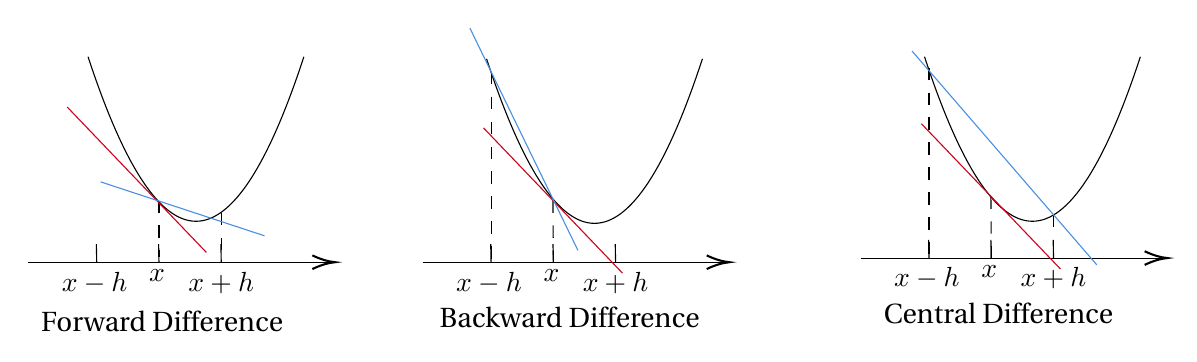
\begin{tikzpicture}[x=0.75pt,y=0.75pt,yscale=-1,xscale=1]
	\draw    (37,240) -- (182.82,240) ;
	\draw [shift={(184.82,240)}, rotate = 180] [color={rgb, 255:red, 0; green, 0; blue, 0 }  ][line width=0.75]    (10.93,-3.29) .. controls (6.95,-1.4) and (3.31,-0.3) .. (0,0) .. controls (3.31,0.3) and (6.95,1.4) .. (10.93,3.29)   ;
	\draw    (99.82,231.27) -- (100,240.27) ;
	\draw    (129.82,231.27) -- (130,240.27) ;
	\draw    (69.82,231.27) -- (70,240.27) ;
	\draw   (65.82,141) .. controls (100.49,246.7) and (135.16,246.7) .. (169.82,141) ;
	\draw    (227,240) -- (372.82,240) ;
	\draw [shift={(374.82,240)}, rotate = 180] [color={rgb, 255:red, 0; green, 0; blue, 0 }  ][line width=0.75]    (10.93,-3.29) .. controls (6.95,-1.4) and (3.31,-0.3) .. (0,0) .. controls (3.31,0.3) and (6.95,1.4) .. (10.93,3.29)   ;
	\draw    (289.82,231.27) -- (290,240.27) ;
	\draw    (319.82,231.27) -- (320,240.27) ;
	\draw    (259.82,231.27) -- (260,240.27) ;
	\draw   (257.82,142) .. controls (292.49,247.7) and (327.16,247.7) .. (361.82,142) ;
	\draw    (438,238) -- (583.82,238) ;
	\draw [shift={(585.82,238)}, rotate = 180] [color={rgb, 255:red, 0; green, 0; blue, 0 }  ][line width=0.75]    (10.93,-3.29) .. controls (6.95,-1.4) and (3.31,-0.3) .. (0,0) .. controls (3.31,0.3) and (6.95,1.4) .. (10.93,3.29)   ;
	\draw    (500.82,229.27) -- (501,238.27) ;
	\draw    (530.82,229.27) -- (531,238.27) ;
	\draw    (470.82,229.27) -- (471,238.27) ;
	\draw   (468.82,141) .. controls (503.49,246.7) and (538.16,246.7) .. (572.82,141) ;
	\draw  [dash pattern={on 4.5pt off 4.5pt}]  (100,210.27) -- (100,237.27) ;
	\draw  [dash pattern={on 4.5pt off 4.5pt}]  (130,216.27) -- (130,240.27) ;
	\draw [color={rgb, 255:red, 208; green, 2; blue, 27 }  ,draw opacity=1 ]   (55.82,165.27) -- (122.82,235.27) ;
	\draw [color={rgb, 255:red, 74; green, 144; blue, 226 }  ,draw opacity=1 ]   (71.82,201.27) -- (150.82,227.27) ;
	\draw  [dash pattern={on 4.5pt off 4.5pt}]  (289.82,210.27) -- (290,240.27) ;
	\draw  [dash pattern={on 4.5pt off 4.5pt}]  (260,148.27) -- (260,240.27) ;
	\draw [color={rgb, 255:red, 208; green, 2; blue, 27 }  ,draw opacity=1 ]   (256.32,175.27) -- (323.32,245.27) ;
	\draw [color={rgb, 255:red, 74; green, 144; blue, 226 }  ,draw opacity=1 ]   (249.82,127.27) -- (301.82,234.27) ;
	\draw  [dash pattern={on 4.5pt off 4.5pt}]  (500.82,208.27) -- (501,238.27) ;
	\draw  [dash pattern={on 4.5pt off 4.5pt}]  (471,146.27) -- (471,238.27) ;
	\draw  [dash pattern={on 4.5pt off 4.5pt}]  (531,217.27) -- (531,238.27) ;
	\draw [color={rgb, 255:red, 208; green, 2; blue, 27 }  ,draw opacity=1 ]   (467.32,173.27) -- (534.32,243.27) ;
	\draw [color={rgb, 255:red, 74; green, 144; blue, 226 }  ,draw opacity=1 ]   (462.82,138.27) -- (551.82,241.27) ;
	\draw (94,242.4) node [anchor=north west][inner sep=0.75pt]    {$x$};
	\draw (112.91,243.4) node [anchor=north west][inner sep=0.75pt]    {$x+h$};
	\draw (51.91,243.4) node [anchor=north west][inner sep=0.75pt]    {$x-h$};
	\draw (284,242.4) node [anchor=north west][inner sep=0.75pt]    {$x$};
	\draw (302.91,243.4) node [anchor=north west][inner sep=0.75pt]    {$x+h$};
	\draw (241.91,243.4) node [anchor=north west][inner sep=0.75pt]    {$x-h$};
	\draw (495,240.4) node [anchor=north west][inner sep=0.75pt]    {$x$};
	\draw (513.91,241.4) node [anchor=north west][inner sep=0.75pt]    {$x+h$};
	\draw (452.91,241.4) node [anchor=north west][inner sep=0.75pt]    {$x-h$};
	\draw (42,262) node [anchor=north west][inner sep=0.75pt]   [align=left] {Forward Difference};
	\draw (234,260.26) node [anchor=north west][inner sep=0.75pt]   [align=left] {Backward Difference};
	\draw (448,258.26) node [anchor=north west][inner sep=0.75pt]   [align=left] {Central Difference};
	\end{tikzpicture}
	\end{center}
\end{df}
\begin{eg}{Finite Difference}
	Suppose $f(x)=x^4$. We want to approximate $f'(1)$. By hand, we know $f'(x)=4x^3$, so $f'(1)=4$. However, numerically, we have the first order approximation ($\bigO(h)$) is \[f'(1)\approx\dsst\dfrac{f(1+h)-f(1)}{h}\] and the second order approximation ($\bigO(h^2)$) is \[f'(1)\approx\dfrac{f(1+h)-f(1-h)}{2h}\] Note that in the first order approximation, every time we divide $h$ by $10$, we are $10$ times more accurate. In the second order approximation, every time we divide $h$ by $10$, we will be $100$ times more accurate. 
\end{eg}
\begin{rmk}
	Why Central Differencing is in Second Order? \par 
	By Taylor series, we know \begin{align*}f(x+h)&=f(x)+f'(x)h+\dfrac{1}{2}f''(x)h^2+\bigO(h^3)\\f(x-h)&=f(x)-f'(x)h+\dfrac{1}{2}f''(x)h^2+\bigO(h^3).\end{align*} Then, \begin{align*}f(x+h)-f(x-h)&=f(x)+f'(x)h+\dfrac{1}{2}f''(x)h^2+\bigO(h^3)\\&\qquad-\qty[f(x)-f'(x)h+\dfrac{1}{2}f''(x)h^2+\bigO(h^3)]\\&=2f'(x)h+\bigO(h^3)\\f'(x)&=\dfrac{f(x+h)-f(x-h)}{2h}+\bigO(h^2)&Divide\ by\ h\\&\approx\dfrac{f(x+h)-f(x-h)}{2h}\end{align*}
\end{rmk}

\subsection{Integration}
\begin{df}{Definite Integral}
	Suppose $f$ is a function defined over the interval $[a,b]$. Then, the functional $I(x)$ is the area under the curve, and \[I(f)=\int_a^bf(x)\ \d{x}.\]
\end{df}
\begin{df}{Functional}
	A functional is a mapping from functions to real numbers.
\end{df}
\begin{thm}{Steps to approximate $I(f)$}
	\begin{itemize}
		\item Partition the Interval: $a\leq x_0<x_1<x_2<\cdots<x_N\leq b$.
		\item Evaluate $f$ at points $x_i$, we get $f(x_i)$ and the data $\qty{(x_i, f_i)}_{i=0}^N$.
		\item Integrate using Riemanian Sums
	\end{itemize}	
\end{thm}
\begin{df}{Midpoint Rule}
	\[\int_{x_{i-1}}^{x_{i}} f(x)\ \d{x}\approx\int_{x_{i-1}}^{x_i}f\qty(\dfrac{x_{i-1}+x_i}{2})\ \d{x}=\qty(x_i-x_{i-1})f\qty(\dfrac{x_{i-1}-x_i}{2}).\]
	\begin{center}
		\tikzset{every picture/.style={line width=0.75pt}} 
		\begin{tikzpicture}[x=0.75pt,y=0.75pt,yscale=-1,xscale=1]
		\draw    (110,250) -- (387.82,250) ;
		\draw [shift={(389.82,250)}, rotate = 180] [color={rgb, 255:red, 0; green, 0; blue, 0 }  ][line width=0.75]    (10.93,-3.29) .. controls (6.95,-1.4) and (3.31,-0.3) .. (0,0) .. controls (3.31,0.3) and (6.95,1.4) .. (10.93,3.29)   ;
		\draw    (160,241.27) -- (160,250.27) ;
		\draw    (200,241.27) -- (200,250.27) ;
		\draw    (240,241.27) -- (240,250.27) ;
		\draw    (280,241.27) -- (280,250.27) ;
		\draw    (320,241.27) -- (320,250.27) ;
		\draw    (160,180.27) .. controls (237,302.27) and (245.82,50.27) .. (319.82,160.27) ;
		\draw  [dash pattern={on 4.5pt off 4.5pt}]  (160,180.27) -- (160,250.27) ;
		\draw  [dash pattern={on 4.5pt off 4.5pt}]  (319.82,160.27) -- (320,250.27) ;
		\draw  [dash pattern={on 4.5pt off 4.5pt}]  (200,214.27) -- (200,250.27) ;
		\draw  [dash pattern={on 4.5pt off 4.5pt}]  (240,176.27) -- (240,250.27) ;
		\draw  [dash pattern={on 4.5pt off 4.5pt}]  (280,132.27) -- (280,250.27) ;
		\draw   (160,206.27) -- (200,206.27) -- (200,250.27) -- (160,250.27) -- cycle ;
		\draw  [fill={rgb, 255:red, 0; green, 0; blue, 0 }  ,fill opacity=1 ] (177.82,205.91) .. controls (177.82,204.76) and (178.76,203.82) .. (179.91,203.82) .. controls (181.06,203.82) and (182,204.76) .. (182,205.91) .. controls (182,207.06) and (181.06,208) .. (179.91,208) .. controls (178.76,208) and (177.82,207.06) .. (177.82,205.91) -- cycle ;
		\draw   (200,205.27) -- (240,205.27) -- (240,250.27) -- (200,250.27) -- cycle ;
		\draw  [fill={rgb, 255:red, 0; green, 0; blue, 0 }  ,fill opacity=1 ] (217.82,204.91) .. controls (217.82,203.76) and (218.76,202.82) .. (219.91,202.82) .. controls (221.06,202.82) and (222,203.76) .. (222,204.91) .. controls (222,206.06) and (221.06,207) .. (219.91,207) .. controls (218.76,207) and (217.82,206.06) .. (217.82,204.91) -- cycle ;
		\draw   (240,146.27) -- (280,146.27) -- (280,250.27) -- (240,250.27) -- cycle ;
		\draw  [fill={rgb, 255:red, 0; green, 0; blue, 0 }  ,fill opacity=1 ] (257.82,146.91) .. controls (257.82,145.76) and (258.76,144.82) .. (259.91,144.82) .. controls (261.06,144.82) and (262,145.76) .. (262,146.91) .. controls (262,148.06) and (261.06,149) .. (259.91,149) .. controls (258.76,149) and (257.82,148.06) .. (257.82,146.91) -- cycle ;
		\draw   (280,138.27) -- (320,138.27) -- (320,250.27) -- (280,250.27) -- cycle ;
		\draw  [fill={rgb, 255:red, 0; green, 0; blue, 0 }  ,fill opacity=1 ] (297.82,137.91) .. controls (297.82,136.76) and (298.76,135.82) .. (299.91,135.82) .. controls (301.06,135.82) and (302,136.76) .. (302,137.91) .. controls (302,139.06) and (301.06,140) .. (299.91,140) .. controls (298.76,140) and (297.82,139.06) .. (297.82,137.91) -- cycle ;
		\draw (152,251.4) node [anchor=north west][inner sep=0.75pt]    {$x_{0}$};
		\draw (191,252.4) node [anchor=north west][inner sep=0.75pt]    {$x_{1}$};
		\draw (231,252.4) node [anchor=north west][inner sep=0.75pt]    {$x_{2}$};
		\draw (271,252.4) node [anchor=north west][inner sep=0.75pt]    {$x_{3}$};
		\draw (311,252.4) node [anchor=north west][inner sep=0.75pt]    {$x_{4}$};
		\end{tikzpicture}
	\end{center}
\end{df}
\begin{df}{Composite Midpoint Rule}
	\begin{align*}I(x)&=\int_a^bf(x)\ \d{x}=\int_{x_0}^{x_1}f(x)\ \d{x}+\int_{x_1}^{x_2}f(x)\ \d{x}+\cdots+\int_{x_{N-1}}^{x_N}f(x)\ \d{x}\\&\approx(x_1-x_0)f\qty(\dfrac{x_0+x_1}{2})+(x_2-x_1)f\qty(\dfrac{x_1+x_2}{2})+\cdots+(x_N-x_{N-1})f\qty(\dfrac{x_{N-1}+x_N}{2})\end{align*} If we have equally spaced points: $x_i=a+ih$ for $i=0,\dots, N$, and $h=\dfrac{b-a}{N}$, then \[I(x)=h\cdot\sum_{i=1}^Nf\qty(x_{\frac{i-1}{2}})\equiv R_{CM}(f,h).\] If $h\to0$, the approximation gets better (in theory). In practice, numerical considerations come into play.	
\end{df}
\begin{df}{Trapezoidal Rule}
	\[\int_{x_{i-1}}^{x_i}f(x)\ \d{x}\approx\qty(x_i-x_{i-1})\qty(\dfrac{f(x_{i-1})+f(x_i)}{2}).\]
	\begin{center}
	\tikzset{every picture/.style={line width=0.75pt}}
	\begin{tikzpicture}[x=0.75pt,y=0.75pt,yscale=-1,xscale=1]
	\draw    (110,250) -- (387.82,250) ;
	\draw [shift={(389.82,250)}, rotate = 180] [color={rgb, 255:red, 0; green, 0; blue, 0 }  ][line width=0.75]    (10.93,-3.29) .. controls (6.95,-1.4) and (3.31,-0.3) .. (0,0) .. controls (3.31,0.3) and (6.95,1.4) .. (10.93,3.29)   ;
	\draw    (160,241.27) -- (160,250.27) ;
	\draw    (200,241.27) -- (200,250.27) ;
	\draw    (240,241.27) -- (240,250.27) ;
	\draw    (280,241.27) -- (280,250.27) ;
	\draw    (320,241.27) -- (320,250.27) ;
	\draw    (160,180.27) .. controls (237,302.27) and (245.82,50.27) .. (319.82,160.27) ;
	\draw    (160,180.27) -- (160,250.27) ;
	\draw    (319.82,160.27) -- (320,250.27) ;
	\draw    (200,214.27) -- (200,250.27) ;
	\draw    (240,176.27) -- (240,250.27) ;
	\draw    (280,132.27) -- (280,250.27) ;
	\draw  [fill={rgb, 255:red, 0; green, 0; blue, 0 }  ,fill opacity=1 ] (157.91,182.36) .. controls (157.91,181.21) and (158.85,180.27) .. (160,180.27) .. controls (161.15,180.27) and (162.09,181.21) .. (162.09,182.36) .. controls (162.09,183.52) and (161.15,184.45) .. (160,184.45) .. controls (158.85,184.45) and (157.91,183.52) .. (157.91,182.36) -- cycle ;
	\draw  [fill={rgb, 255:red, 0; green, 0; blue, 0 }  ,fill opacity=1 ] (197.91,214.27) .. controls (197.91,213.12) and (198.85,212.18) .. (200,212.18) .. controls (201.15,212.18) and (202.09,213.12) .. (202.09,214.27) .. controls (202.09,215.43) and (201.15,216.36) .. (200,216.36) .. controls (198.85,216.36) and (197.91,215.43) .. (197.91,214.27) -- cycle ;
	\draw  [fill={rgb, 255:red, 0; green, 0; blue, 0 }  ,fill opacity=1 ] (237.91,176.27) .. controls (237.91,175.12) and (238.85,174.18) .. (240,174.18) .. controls (241.15,174.18) and (242.09,175.12) .. (242.09,176.27) .. controls (242.09,177.43) and (241.15,178.36) .. (240,178.36) .. controls (238.85,178.36) and (237.91,177.43) .. (237.91,176.27) -- cycle ;
	\draw  [fill={rgb, 255:red, 0; green, 0; blue, 0 }  ,fill opacity=1 ] (277.91,132.27) .. controls (277.91,131.12) and (278.85,130.18) .. (280,130.18) .. controls (281.15,130.18) and (282.09,131.12) .. (282.09,132.27) .. controls (282.09,133.43) and (281.15,134.36) .. (280,134.36) .. controls (278.85,134.36) and (277.91,133.43) .. (277.91,132.27) -- cycle ;
	\draw  [fill={rgb, 255:red, 0; green, 0; blue, 0 }  ,fill opacity=1 ] (317.73,160.27) .. controls (317.73,159.12) and (318.67,158.18) .. (319.82,158.18) .. controls (320.98,158.18) and (321.91,159.12) .. (321.91,160.27) .. controls (321.91,161.43) and (320.98,162.36) .. (319.82,162.36) .. controls (318.67,162.36) and (317.73,161.43) .. (317.73,160.27) -- cycle ;
	\draw    (162.09,182.36) -- (200,216.36) ;
	\draw    (200,214.27) -- (240,176.27) ;
	\draw    (240,176.27) -- (280,132.27) ;
	\draw    (280,132.27) -- (319.82,160.27) ;
	\draw (152,251.4) node [anchor=north west][inner sep=0.75pt]    {$x_{0}$};
	\draw (191,252.4) node [anchor=north west][inner sep=0.75pt]    {$x_{1}$};
	\draw (231,252.4) node [anchor=north west][inner sep=0.75pt]    {$x_{2}$};
	\draw (271,252.4) node [anchor=north west][inner sep=0.75pt]    {$x_{3}$};
	\draw (311,252.4) node [anchor=north west][inner sep=0.75pt]    {$x_{4}$};
	\end{tikzpicture}
	\end{center}
\end{df}
\begin{df}{Composite Trapezoidal Rule}
	\[R_{CT}(f,h)\equiv h\sum_{i=1}^N\qty(\dfrac{f(x_{i-1})+f(x_i))}{2})\]	
\end{df}
\begin{df}{Quadrature Rule}
	The Quadrature question concerns ``Can we find a square that has the same area as a circle?'' In the integration problem, the Quadrature Rules states that given points $x_0<x_1<\cdots<x_N$ and weights $w_0,w_1,\dots,w_N$, then \[R(f)\equiv\sum_{i=0}^N w_if(x_i).\]	
\end{df}
\begin{thm}{Properties of $R(f)$}
	\begin{itemize}
		\item Linear functional: \[R(\alpha f+\beta g)=\alpha R(f)+\beta R(g).\]
		\item Alternative perspective: \[R(f)=I(q),\] where $q$ is an approximation ($q$ has a polynomial interpolant) to $f$. \begin{align*}I(q)&=I(f+(q-f))\\&=I(f)+\underbrace{I(q-f)}_\text{error of integration}\end{align*} Then, the error of integration depends on how well $q$ approximates $f$.
	\end{itemize}	
\end{thm}
\begin{eg}{Midpoint Rule Revisit}
	Use degree $0$ approximation of $f(x)$, $q_0(x)$, and use $x=\dfrac{c+d}{2}$ on $[c,d]$. Then, we have exactly the midpoint rule: 
	\begin{center}
	\tikzset{every picture/.style={line width=0.75pt}}
	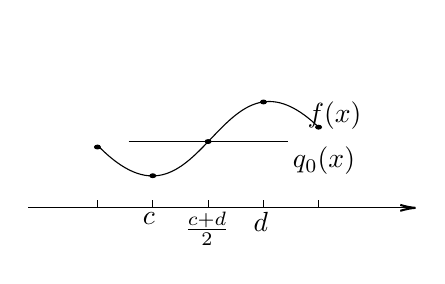
\begin{tikzpicture}[x=0.5pt,y=0.65pt,yscale=-.5,xscale=1]
	\draw    (110,250) -- (387.82,250) ;
	\draw [shift={(389.82,250)}, rotate = 180] [color={rgb, 255:red, 0; green, 0; blue, 0 }  ][line width=0.75]    (10.93,-3.29) .. controls (6.95,-1.4) and (3.31,-0.3) .. (0,0) .. controls (3.31,0.3) and (6.95,1.4) .. (10.93,3.29)   ;
	\draw    (160,241.27) -- (160,250.27) ;
	\draw    (200,241.27) -- (200,250.27) ;
	\draw    (240,241.27) -- (240,250.27) ;
	\draw    (280,241.27) -- (280,250.27) ;
	\draw    (320,241.27) -- (320,250.27) ;
	\draw    (160,180.27) .. controls (237,302.27) and (245.82,50.27) .. (319.82,160.27) ;
	\draw    (182.59,176.27) -- (297.41,176.27) ;
	\draw  [fill={rgb, 255:red, 0; green, 0; blue, 0 }  ,fill opacity=1 ] (157.91,182.36) .. controls (157.91,181.21) and (158.85,180.27) .. (160,180.27) .. controls (161.15,180.27) and (162.09,181.21) .. (162.09,182.36) .. controls (162.09,183.52) and (161.15,184.45) .. (160,184.45) .. controls (158.85,184.45) and (157.91,183.52) .. (157.91,182.36) -- cycle ;
	\draw  [fill={rgb, 255:red, 0; green, 0; blue, 0 }  ,fill opacity=1 ] (197.91,214.27) .. controls (197.91,213.12) and (198.85,212.18) .. (200,212.18) .. controls (201.15,212.18) and (202.09,213.12) .. (202.09,214.27) .. controls (202.09,215.43) and (201.15,216.36) .. (200,216.36) .. controls (198.85,216.36) and (197.91,215.43) .. (197.91,214.27) -- cycle ;
	\draw  [fill={rgb, 255:red, 0; green, 0; blue, 0 }  ,fill opacity=1 ] (237.91,176.27) .. controls (237.91,175.12) and (238.85,174.18) .. (240,174.18) .. controls (241.15,174.18) and (242.09,175.12) .. (242.09,176.27) .. controls (242.09,177.43) and (241.15,178.36) .. (240,178.36) .. controls (238.85,178.36) and (237.91,177.43) .. (237.91,176.27) -- cycle ;
	\draw  [fill={rgb, 255:red, 0; green, 0; blue, 0 }  ,fill opacity=1 ] (277.91,132.27) .. controls (277.91,131.12) and (278.85,130.18) .. (280,130.18) .. controls (281.15,130.18) and (282.09,131.12) .. (282.09,132.27) .. controls (282.09,133.43) and (281.15,134.36) .. (280,134.36) .. controls (278.85,134.36) and (277.91,133.43) .. (277.91,132.27) -- cycle ;
	\draw  [fill={rgb, 255:red, 0; green, 0; blue, 0 }  ,fill opacity=1 ] (317.73,160.27) .. controls (317.73,159.12) and (318.67,158.18) .. (319.82,158.18) .. controls (320.98,158.18) and (321.91,159.12) .. (321.91,160.27) .. controls (321.91,161.43) and (320.98,162.36) .. (319.82,162.36) .. controls (318.67,162.36) and (317.73,161.43) .. (317.73,160.27) -- cycle ;
	\draw (191,252.4) node [anchor=north west][inner sep=0.75pt]    {$c$};
	\draw (221,251.4) node [anchor=north west][inner sep=0.75pt]    {$\frac{c+d}{2}$};
	\draw (271,252.4) node [anchor=north west][inner sep=0.75pt]    {$d$};
	\draw (310,129.4) node [anchor=north west][inner sep=0.75pt]    {$f( x)$};
	\draw (299.41,179.67) node [anchor=north west][inner sep=0.75pt]    {$q_{0}( x)$};
	\end{tikzpicture}
	\end{center}
\end{eg}
\begin{eg}{Trapezoidal Rule Revisit}
	Use degree $1$ approximation of $f(x)$, $q_1(x)$, with $q_1(c)=f(c)$ and $q_1(d)=f(d)$: 
	\begin{center}	
	\tikzset{every picture/.style={line width=0.75pt}}
	\begin{tikzpicture}[x=0.5pt,y=0.5pt,yscale=-1,xscale=1]
	\draw    (110,250) -- (387.82,250) ;
	\draw [shift={(389.82,250)}, rotate = 180] [color={rgb, 255:red, 0; green, 0; blue, 0 }  ][line width=0.75]    (10.93,-3.29) .. controls (6.95,-1.4) and (3.31,-0.3) .. (0,0) .. controls (3.31,0.3) and (6.95,1.4) .. (10.93,3.29)   ;
	\draw    (200,241.27) -- (200,250.27) ;
	\draw    (280,241.27) -- (280,250.27) ;
	\draw    (160,180.27) .. controls (237,302.27) and (245.82,50.27) .. (319.82,160.27) ;
	\draw    (200,214.27) -- (280,132.27) ;
	\draw  [fill={rgb, 255:red, 0; green, 0; blue, 0 }  ,fill opacity=1 ] (197.91,214.27) .. controls (197.91,213.12) and (198.85,212.18) .. (200,212.18) .. controls (201.15,212.18) and (202.09,213.12) .. (202.09,214.27) .. controls (202.09,215.43) and (201.15,216.36) .. (200,216.36) .. controls (198.85,216.36) and (197.91,215.43) .. (197.91,214.27) -- cycle ;
	\draw  [fill={rgb, 255:red, 0; green, 0; blue, 0 }  ,fill opacity=1 ] (277.91,132.27) .. controls (277.91,131.12) and (278.85,130.18) .. (280,130.18) .. controls (281.15,130.18) and (282.09,131.12) .. (282.09,132.27) .. controls (282.09,133.43) and (281.15,134.36) .. (280,134.36) .. controls (278.85,134.36) and (277.91,133.43) .. (277.91,132.27) -- cycle ;
	\draw (191,252.4) node [anchor=north west][inner sep=0.75pt]    {$c$};
	\draw (271,252.4) node [anchor=north west][inner sep=0.75pt]    {$d$};
	\draw (310,129.4) node [anchor=north west][inner sep=0.75pt]    {$f( x)$};
	\draw (257.41,153.67) node [anchor=north west][inner sep=0.75pt]    {$q_{1}( x)$};
	\end{tikzpicture}
	\end{center}
	Use Lagrange polynomials to build $q_1(x)$: \[\l_1(x)=\dfrac{x-d}{c-d},\quad\l_2=\dfrac{x-c}{d-c},\quad q_1(x)=f(c)\l_0(x)+f(d)\l_1(x).\] Then, \begin{align*}I(f)&\approx I(q_1)\\&=f(c)I(\l_0)+f(d)I(\l_1)&Compare:\ w_0f(x_0)+w_1f(x_1)\\&=f(c)\qty(\dfrac{d-c}{2})+f(d)\qty(\dfrac{d-c}{2})\\&=(d-c)\qty(\dfrac{f(c)+f(d)}{2}),\end{align*} which is exactly the trapezoidal rule.
\end{eg}
\begin{df}{Interpolatory Quadrature}
	Given data $\qty{(x_i,f_i)}_{i=0}^N$, ordering $x_0<x_1<\cdots<x_N$, and the interpolating polynomial $q_N(x)$. We can always write \[R(f)=q_N(x)=\sum_{i=0}^Nf(x_i)\l_i(x),\] where $\l_i(x)$'s are Lagrange polynomials: \begin{align*}I(f)\approx R(f)&=I(q_N)\\&=I\qty(\sum_{i=0}^N\underbrace{f(x_i)}_\text{constant}\overbrace{\l_i(x)}^\text{variable})\\&=\sum_{i=0}^Nf(x_i)\underbrace{I(\l_i)}_{w_i}&Integration\ is\ a\ linear\ functional\end{align*} So, $w_i=I(\l_i)=\dsst\int_a^b\l_i(x)\ \d{x}$.
\end{df}
\begin{df}{Newton-Cotes Rules}
	We are working with interpolatory quadrature with equally spaced points. That is, $x_1=a+ih$ and $h=(b-a)/N$. We have two types of Newton-Cotes Rules: 
	\begin{itemize}
		\item Closed $(N+1)$-point Newton-Cotes: We will use all points $x_0,\dots,x_N$, including endpoints.
		\item Open $(N-1)$-point Newton-Cotes: Use only interior points: $x_1,\dots,x_{N-1}$.
	\end{itemize}
\end{df}
\begin{eg}{Midpoint Rule and Trapezoidal Rule as Newton-Cotes}
	The midpoint rule is equivalent to an open $1$-point Newton Cotes. On the other hand, the trapezoidal rule is equivalent to a closed $2$-point Newton-Cotes. 
	\begin{center}
	\tikzset{every picture/.style={line width=0.75pt}}
	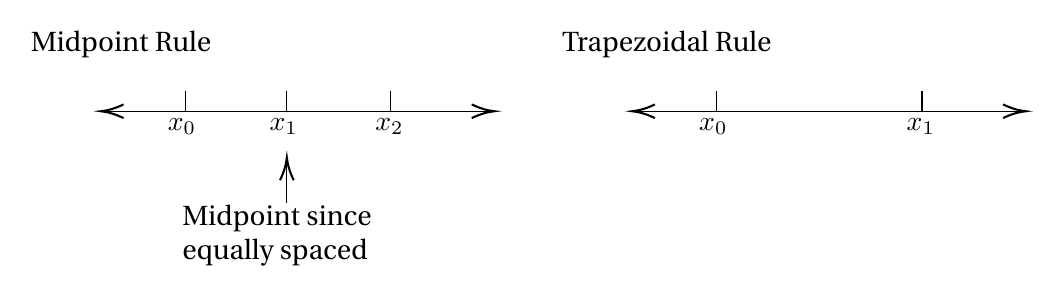
\begin{tikzpicture}[x=0.75pt,y=0.75pt,yscale=-1,xscale=1]
	\draw    (102,100) -- (287.6,100) ;
	\draw [shift={(289.6,100)}, rotate = 180] [color={rgb, 255:red, 0; green, 0; blue, 0 }  ][line width=0.75]    (10.93,-3.29) .. controls (6.95,-1.4) and (3.31,-0.3) .. (0,0) .. controls (3.31,0.3) and (6.95,1.4) .. (10.93,3.29)   ;
	\draw [shift={(100,100)}, rotate = 0] [color={rgb, 255:red, 0; green, 0; blue, 0 }  ][line width=0.75]    (10.93,-3.29) .. controls (6.95,-1.4) and (3.31,-0.3) .. (0,0) .. controls (3.31,0.3) and (6.95,1.4) .. (10.93,3.29)   ;
	\draw    (140.6,100.3) -- (140.6,90.3) ;
	\draw    (189.6,100.3) -- (189.6,90.3) ;
	\draw    (239.6,100.3) -- (239.6,90.3) ;
	\draw    (358,100) -- (543.6,100) ;
	\draw [shift={(545.6,100)}, rotate = 180] [color={rgb, 255:red, 0; green, 0; blue, 0 }  ][line width=0.75]    (10.93,-3.29) .. controls (6.95,-1.4) and (3.31,-0.3) .. (0,0) .. controls (3.31,0.3) and (6.95,1.4) .. (10.93,3.29)   ;
	\draw [shift={(356,100)}, rotate = 0] [color={rgb, 255:red, 0; green, 0; blue, 0 }  ][line width=0.75]    (10.93,-3.29) .. controls (6.95,-1.4) and (3.31,-0.3) .. (0,0) .. controls (3.31,0.3) and (6.95,1.4) .. (10.93,3.29)   ;
	\draw    (396.6,100.3) -- (396.6,90.3) ;
	\draw    (495.6,100.3) -- (495.6,90.3) ;
	\draw    (189.6,144.3) -- (189.6,124.3) ;
	\draw [shift={(189.6,122.3)}, rotate = 90] [color={rgb, 255:red, 0; green, 0; blue, 0 }  ][line width=0.75]    (10.93,-3.29) .. controls (6.95,-1.4) and (3.31,-0.3) .. (0,0) .. controls (3.31,0.3) and (6.95,1.4) .. (10.93,3.29)   ;
	\draw (131,102.4) node [anchor=north west][inner sep=0.75pt]    {$x_{0}$};
	\draw (180,102.4) node [anchor=north west][inner sep=0.75pt]    {$x_{1}$};
	\draw (231,102.4) node [anchor=north west][inner sep=0.75pt]    {$x_{2}$};
	\draw (138,144) node [anchor=north west][inner sep=0.75pt]   [align=left] {Midpoint since \\equally spaced};
	\draw (65,60) node [anchor=north west][inner sep=0.75pt]   [align=left] {Midpoint Rule};
	\draw (387,102.4) node [anchor=north west][inner sep=0.75pt]    {$x_{0}$};
	\draw (487,102.4) node [anchor=north west][inner sep=0.75pt]    {$x_{1}$};
	\draw (321,60) node [anchor=north west][inner sep=0.75pt]   [align=left] {Trapezoidal Rule};
	\end{tikzpicture}
	\end{center}
\end{eg}
\begin{thm}{Simpson's Rule}
	The Simpsons's Rule is a closed $3$-point Newton-Cotes. The Simpson's Rule states that \[I(f)=\int_a^bf(x)\ \d{x}\approx\dfrac{b-a}{6}\qty[f(a)+4f\qty(\dfrac{a+b}{2})+f(b)].\]	
\end{thm}
\begin{prf}
	\begin{align*}w_0&=\dfrac{b-a}{6}=\int_a^b\l_0(x)\ \d{x}=\int_a^b\dfrac{\qty(x-\frac{a+b}{2})(x-b)}{\qty(a-\frac{a+b}{2})(a-b)}\ \d{x}\\w_1&=\dfrac{4(b-a)}{6}=\int_a^b\l_1(x)\ \d{x}\\w_2&=\dfrac{b-a}{6}=\int_a^b\l_2(x)\ \d{x}\end{align*}
\end{prf}

\subsection{Error in Integration}
\begin{thm}{Integral Mean Value Theorem}
	Suppose $g(x)$ and $w(x)$ are continuous on $[a,b]$, and $w(x)$ is non-negative on $(a,b)$. Then, for some point $\eta\in(a,b)$, we get \[\int_a^b\underbrace{w(x)}_\text{weight}g(x)\ \d{x}=\qty{\int_a^bw(x)\ \d{x}}g(\eta).\]	
\end{thm}
\begin{prf}
	Since $g(x)$ is continuous on $[a,b]$, by the Extreme Value Theorem, $g(x)$ attains a maximum and minimum on $[a,b]$. Let $\dsst m=\min_{x\in[a,b]}g(x)$ and $M=\dsst\max_{x\in[a,b]}g(x)$. Then, since $w(x)\geq0\quad\forall x\in(a,b)$, we have \[m\int_a^bw(x)\ \d{x}\leq\int_a^b w(x)g(x)\ \d{x}\leq M\int_a^bw(x)\ \d{x}.\] Since $g(x)$ is continuous on $[a,b]$, by the Intermediate Value Theorem, $g(x)$ attains every value between $m$ and $M$. In other words, for any $y\st m\leq y\leq M,\ \exists\eta\st g(\eta)=y$. Therefore, $\exists\eta\in(a,b)\st$ the statement holds. 
\end{prf}
\begin{thm}{Error in Trapezoidal Rule}
	\[I(f)-R_T(f)=-\dfrac{(d-c)^3}{12}f''(\eta)\quad\text{for some}\ \eta\in(a,b)\]	
\end{thm}
\begin{prf}
	The error in trapezoidal rule is given by \begin{align*}I(f)-R_T(f)&=I(f)-I(q_1)&q_1\ is\ a\ linear\ approximation\\&=I(f-q_1)\\&=\int_c^d\qty{\text{error in linear interpolation}}\ \d{x}\end{align*} So, error in integration is the integral of error in interpolation. Recall \[f(x)-q_1(x)=\dfrac{\omega(x)}{2!}f''(\xi_x),\text{ where }\omega(x)=(x-c)(x-d).\] Then, \begin{align*}I(f)-R_T(f)&=\int_c^d\underbrace{\dfrac{(x-c)(x-d)}{2}}_{w(x)}\underbrace{f''(\xi_x)}_{g(x)}\ \d{x}\\&=-\int_c^d\dfrac{(x-c)(d-x)}{2}f''(\xi_x)\ \d{x}\\&=-\qty{\int_c^d\dfrac{(x-c)(d-x)}{2}\ \d{x}}f''(\eta)\\&=-\dfrac{(d-c)^3}{2}f''(\eta).\end{align*}
\end{prf}
\begin{cor}{}
	If $f''(\eta)\geq0$, then we always overestimate the integral since the error is negative. If $f''(\eta)<0$, then we always underestimate the integral since error is positive. 
\end{cor}
\begin{thm}{Errors in Composite Trapozoidal Rule}
	\[I(f)-R_{CT}(f,h)=-\dfrac{h^3}{12}Nf''(\eta)=-\dfrac{h^2}{12}\underbrace{(b-a)}_{=Nh}f''(\eta),\quad N=\text{ \# of intervals}\]
\end{thm}
\begin{thm}{Errors in Midpoint Rule and Composite Midpoint Rule}
	\[I(f)-R_M(f)=\dfrac{(d-c)^3}{24}f''(\eta);\]
	\[I(f)-R_{CM}(f)=\dfrac{h^3}{24}Nf''(\eta)=\dfrac{h^2}{24}(b-a)f''(\eta).\]	
\end{thm}
\begin{df}{Degree of Precision/DOP}
	We say $R(f)$ has $\DOP=m$ if \[R(p_k)=I(p_k)\quad\text{for }k=0,1,\dots,m,\] and \[R(p_{m+1})\neq I(p_{m+1}).\]
\end{df}
\begin{thm}{DOP Test}
	$R(f)$ has a $\DOP=m$ if $R(x^k)=I(x^k)$ for $k=0,1,\dots,m$ and $R\qty(x^{m+1})\neq I\qty(x^{m+1})$.
\end{thm}
\begin{eg}{DOP of Midpoint Rule, Trapezoidal Rule, and Simpson's Rule}
	\begin{itemize}
		\item Midpoint rule has $\DOP=1$.
		\begin{prf}\begin{center}\begin{tabular}{c|c|c|c}
			$k$&degree $k$&$I\qty(x^k)$&$R\qty(x^k)$\\\hline
			$0$&$p_0(x)=1$&$\dsst\int_a^b1\ \d{x}=b-a$&$(b-a)(1)$\\
			$1$&$p_1(x)=x$&$\dsst\int_a^bx\ \d{x}=\frac{1}{2}\qty(b^2-a^2)$&$(b-a)\qty(\frac{a+b}{2})=\frac{1}{2}\qty(b^2-a^2)$\\
			$2$&$p_2(x)=x^2$&$\dsst\int_a^bx^2\ \d{x}=\dfrac{1}{3}\qty(b^3-a^3)$&$(b-a)\qty(\dfrac{a+b}{2})^2=\dfrac{1}{4}(a+b)^2(b-a)$
		\end{tabular}\end{center} So, the Midpoint Rule has a $\DOP=1$.\end{prf}
		\begin{rmk}
			Super-convergence in Midpoint Rule:	we use a degree $0$ polynomial to interpolate our data, but we end up with a $\DOP=1>0$.
		\end{rmk}
		\item Trapezoidal Rule has a $\DOP=1$.
		\item Simpson's Rule has a $\DOP=3$. (Super-convergence)
	\end{itemize}
\end{eg}
\begin{rmk}Super-convergence generally means we use a bad interpolation but get an accurate approximation of integral. (Degree of interpolation $<\DOP$)\end{rmk}
\begin{thm}{Method of Underdetermined Coefficient}
	Goal: maximize $\DOP$ by choosing weights (given $x_0,\dots,x_N$ on canonical interval $[-1,1]$). When $k=0$, we have \[\int_{-1}^11\ \d{x}=\sum_{i=0}^Nw_i(1)\quad\DOP\geq0\] When $k=1$, we have \[\int_{-1}^1x\ \d{x}=\sum_{i=0}^Nw_ix_i\quad\DOP\geq1\] \[\vdots\] When $k=m$, we have \[\int_{-1}^1x^m\ \d{x}=\sum_{i=0}^Nw_ix_i^m\quad\DOP\geq m\] If the next equation is not satisfied, $\DOP=,$. That is, \[\int_{-1}^1x^{m+1}\ \d{x}\neq\sum_{i=0}^Nw_ix_i^{m+1}\] We now have $m+1$ equations and $N+1$ unknowns ($w_0,\dots,w_N$). To find the weights, we solve a linear system. 
\end{thm}
\begin{eg}{Method of Underdetermined Coefficients}
	Suppose $x_0=-1,\ x_1=0,\ x_2=+1$. Develop a $R(f)=w_0f(-1)+w_1f(0)+w_2f(+1)$.
	\begin{sol}\begin{center}\begin{tabular}{c|c|c|c}
		$k$&degree $k$&$I\qty(x^k)$&$R\qty(x^k)$\\\hline
		$0$&$p_0(x)=1$&$\dsst\int_{-1}^11\ \d{x}=2$&$w_0+w_1+w_2$\\
		$1$&$p_1(x)=x$&$\dsst\int_{-1}^1x\ \d{x}=0$&$-w_0+w_2$\\
		$2$&$p_2(x)=x^2$&$\dsst\int_{-1}^1x^2\ \d{x}=\dfrac{2}{3}$&$w_0+w_2$\\
		$3$&$p_3(x)=x^3$&$\dsst\int_{-1}^1x^3\ \d{x}=0$&$-w_0+w_2$\\
		$4$&$p_4(x)=x^4$&$\dsst\int_{-1}^1x^4\ \d{x}=\dfrac{2}{5}$&$w_0+w_2$
	\end{tabular}\end{center} So, we  can form the following system of equations: \[\begin{cases}w_0+w_1+w_2=2\\-w_0+w_2=0\\w_0+w_2=2/3\end{cases}\implies\begin{cases}w_0=1/3\\w_1=4/3\\w_2=1/3\end{cases}\] Therefore, we have a $\DOP=3$, which is a case of superconvergence. \[R(f)=\dfrac{(+1)-(-1)}{6}\qty\Big[f(-1)+4f(0)+f(1)]\longrightarrow\text{Simpson's Rule}\]\end{sol}
\end{eg}
\begin{thm}{Peano's Theorem}
	Suppose
	\begin{itemize}
		\item $R(f)$ with $\DOP=m$, and 
		\item integrand $f(x)$ and its first $m+1$ derivatives exist and are continuous on $[a,b]$.
	\end{itemize}
	Then, there exists a function $K(x)$, the Peano's Kernel, for which \[I(f)-R(f)=\int_a^bK(x)f^{(m+1)}(x)\ \d{x}\]
\end{thm}
\begin{cor}{}
	If $K(x)$ does not change sign on $[a,b]$, then by the Integral Mean Value Theorem, we get \[I(f)-R(f)=\kappa f^{(m+1)}(\eta),\] for some $\eta\in(a,b)$ and $\kappa$ is a number called the \textit{Peano's constant}. 
	\begin{rmk} Midpoint Rule, Trapezoidal Rule, Simpson's Rule satisfy the condition that $K(x)$ does not change sign on $[a,b]$.\end{rmk}
\end{cor}
\begin{eg}{Peano's Kernel}
	On $[-1,1]$, the Simpson's Rule gives us \[R(f)=\dfrac{1}{3}\qty\Big[f(-1)+4f(0)+f(1)],\] with $\DOP=3$. Then, by Peano's Theorem, \[I(f)-R(f)=\int_{-1}^1K(x)f^{(4)}(x)\ \d{x}=\kappa f^{(4)}(\eta).\] Estimate the Peano's constant $\kappa$.
	\begin{sol}
		Choose $f(x)=x^4$, so we have $f^{(4)}(x)=24$. Then \[I(x^4)-R(x^4)=\kappa f^{(4)}(\eta)\implies\dfrac{2}{5}-\dfrac{2}{3}=24\kappa\implies\kappa=-\dfrac{1}{90}\]
	\end{sol}
\end{eg}

\subsection{Adaptive Integration and More}
\begin{thm}{Characteristics of Adaptive Integration}
	\begin{itemize}
		\item Fewer function evaluations
		\item Control of error
		\item Goal: estimate $\dsst I(f,T)\equiv\int_Tf(x)\ \d{x}$, where $T=[a,b]$.
	\end{itemize}	
\end{thm}
\begin{nota}
	$T^*$: subinterval of $T$. $R_1(f,T^*)$ and $R_2(f,T^*)$ are both quadrature rules, but $R_2$ is more accurate (with higher $\DOP$/composite method). 
\end{nota}
\begin{df}{Etimate Error}
	\begin{align*}E(f,T^*)&=\qty|I(f,T^*)-R_1(f,T^*)|\\&\approx\qty|R_2(f,T^*)-R_1(f,T^*)|\end{align*}
\end{df}
\begin{algorithm}\caption{Adaptive Integration}
	Partition $T$ into subintervals $T_i$, where $i=1,\dots,n$;\\
	Compute	$R(f,T_i)$ and $E(f,T_i)$ for $i=1,\dots,n$;\\
	Find the subinterval with largest error and bisect. Say $T_{i^*}$ is the interval, then we turn it into $T_{i^*}^\text{left}$ and $T_{i^*}^\text{right}$;\\
	Repeat. Stop when we get $\dsst\sum_{i=1}^nE(f,T_i)\leq\underbrace{\text{tolerance}}_\text{to be chosen}$;
\end{algorithm}
\begin{df}{Gauss Rules}
	\begin{itemize}
		\item Main idea: maximize $\DOP$ by choosing weights $w_i$ and nodes $x_i$.
		\item Assumption: canonical interval $[-1,1]$.
		\item Properties:
		\begin{itemize}
			\item positive weights: $w_i>0$
			\item interior nodes: $x_i\in(-1,1)$ for $i=0,\dots,N$
			\item symmetry
			\item interlacing: when comparing $N$-point and $(N+1)$-point, those nodes will appear in the interweaving/interlacing order. \textit{This guarantees good sampling of integration intervals}
			\item interpolatory
			\item $\DOP$ of $(N+1)$-point Gauss Quadrature is $2N+1$.
		\end{itemize}
	\end{itemize}
\end{df}
\begin{rmk}
	There are other rules such as Lobatto Rules or Gauss-Kronrod Rules. They are also widely used in practice.	
\end{rmk}
\begin{thm}{Transformation from Canonical Interval}
	\[\int_{g(c)}^{g(d)}f(x)\ \d{x}=\int_c^df(g(t))g'(t)\ \d{t},\]	where $f(g(t))$ represents evaluating $f$ on $[a,b]$, and $g'(t)$ shows how much $[a,b]$ is stretched/shrunk from $[-1,1]$. In our case, $c=-1,\ d=+1,$ and $g:[-1,1]\to[a,b]$. We will use a linear map that maps $-1$ to $a$ and $+1$ to $b$: \[g(t)=\dfrac{(b-a)}{2}t+\dfrac{(b+a)}{2}\] So, \begin{align*}I(f)\equiv\int_a^bf(x)\ \d{x}&=\underbrace{\dfrac{b-a}{2}}_{g'(t)}\int_{-1}^1f\qty(\dfrac{b-a}{2}t+\dfrac{b+a}{2})\ \d{t}\\&\approx\dfrac{b-a}{2}\sum_{i=0}^Nw_i^*f\qty(\dfrac{b-a}{2}t_i^*+\dfrac{b+a}{2})\\&=\sum_{i=0}^Nw_if(x_i),\end{align*} where $w_i=\dfrac{b-a}{2}w_i^*$ and $x_i=\dfrac{b-a}{2}t_i^*+\dfrac{b+a}{2}$.

\end{thm}

\newpage
\section{Root Finding}
\subsection{Fixed Point Iteration (FPI)}
\begin{df}{Root}
	A \textit{root} of a function $f$ is a point $x_*$ where $f(x_*)=0$.	
\end{df}
\begin{df}{Simple Root}
	A point $x_*$ is a \textit{simple root} of a function $f$ if the following hold: 
	\begin{itemize}
		\item $x_*$ is a root, i.e.,  $f(x_*)=0$,
		\item $f'(x)$ exists everywhere on an open interval containing $x_*$, and
		\item $f'(x_*)\neq0$.
	\end{itemize}	
\end{df}
\begin{rmk}
	 In other words, we corss the $x$-axis ``like a line.''	
\end{rmk}
\begin{df}{Fixed Point}
	A point $x_*$ is a \textit{fixed point} of function $g$ if $x_*=g(x_*)$.	
\end{df}
\begin{rmk}
	It is those points where $g(x)$ intersects $y=x$.	
\end{rmk}
\begin{thm}{Fixed Point and Root}
	If $x_*$ is a fixed point of $g$, then $x_*$ is a root of $f(x)=x-g(x)$. Conversely, if $x_*$ is a root of $f(x)$, then $x_*$ is a fixed point of $g(x)=x-f(x)$. 
\end{thm}
\begin{eg}{}
	Given $g(x)=5-\dfrac{3}{x+2}$. Find fix points of this function.
	\begin{sol}
		\[x=g(x)\implies x=5-\dfrac{3}{x+2}\implies x^2-3x+7=0\implies x_*=\dfrac{3\pm\sqrt{37}}{2}\]
	\end{sol}
\end{eg}
\begin{algorithm}\caption{Fixed Point Iteration (FPI)}
	Goal: Find $x_*$ such that $x_*=g(x_*)$\;
	Start with a guess $x_0$. Repeat the following step: \[x_{n+1}=g(x_n),\quad n=0,1,\dots,\] where $g$ is the FPI function\;
\end{algorithm}
\begin{rmk} The result of FPI depends significantly on our initial guess! \end{rmk}
\begin{eg}{}
	Find fixed points of $g(x)=e^{-x}$.\par 
	Guess: $x_0=0.5$. Then, \[x_1=g(x_0)=g(0.5)\approx0.6065;\quad x_2=g(x_1)=g(0.6065)\approx0.5452;\dots\]
\end{eg}
\begin{rmk}
	Consider $h(x)=-\ln(x)$. $x_*$ of $g(x)$ is also a fixed point of $h(x)$: \[x_*=g(x_*)=e^{x_*}\implies\ln(x_*)=-x_*\implies x_*=-\ln(x_*)=h(x_*).\] However, using the guess $x_0=0.5$ to solve for a fixed point of $h(x)$ would not result in a converging fixed point. 
\end{rmk}

\subsection{Convergence Iteration Analysis}
\begin{df}{Error}
	The \textit{err}r of FPI is defined as \[e_n\coloneqq x_n-x_*\]	
\end{df}
\begin{thm}{}
	If FPI converges, then $\qty{\qty|e_n|}_{n=0}^\infty$ decreases monotonically eventually. 
\end{thm}
\begin{rmk}
	We will assume $g'(x)$ is continuous whenever we need. 	
\end{rmk}
\begin{thm}{Mean Value Theorem, MVT}
	By the mean value theorem, we can find the relationship between $e_{n+1}$ and $e_n$.
	\begin{align*}
		e_{n+1}&=x_{n+1}-x_*\\&=g(x_n)-g(x_*)\\&=g'(\eta_n)(x_n-x_*)\\e_{n+1}&=g'(\eta_n)e_n
	\end{align*}	
\end{thm}
\begin{thm}{Convergence Analysis}
	We have $\qty|e_{n+1}|<\qty|e_n|\iff\qty|g'(\eta_n)|\leq G<1$.	
\end{thm}
\begin{thm}{Tangent Line Condition}
	If $\qty|g'(x)|\leq G<1\quad\forall x\in I=[x_*-r,x_*+r]$, then FPI converges for every starting guess $x_i\in I$.	
\end{thm}
\begin{cor}{}
	If $g'(x_*)>0$, convergence is on-sided ($=$ the sign of error does not change). If $g'(x_*)<0$, convergence is two-sided ($=$ the sign of error changes).
\end{cor}
\begin{thm}{}
	 The smaller $\qty|g'(x_*)|$, the faster we converge.	
\end{thm}
\begin{thm}{Error Approximation}
	When $x_n$ is close enough to $x_*$, \[e_{n+1}\approx g'(x_*)e_n\]	
\end{thm}
\begin{df}{Linear, Superlinear}
	Convergence rate is \textit{linear} if $g'(x_*)\neq0$. Convergence rate is \textit{superlinear} if $g'(x_*)=0$.
\end{df}
\begin{df}{Convergence Rate}
	If $\dsst\lim_{n\to\infty}\dfrac{\qty|e_{n+1}|}{\qty|e_n|^p}=K$, where $K>0$, then the \textit{convergence rate} is \textit{order-$p$}. If $p=1$ and $K<1$, then convergence is \textit{linear}. If $p=2$, then we have \textit{quadratic convergence}.
\end{df}

\subsection{Root Finding Methods}
\begin{algorithm}
	\caption{Newton Iteration}
	To find a simple root $f(x)=0$, we can use the FPI function \[g(x)=x-\dfrac{f(x)}{f'(x)},\] and apply the fixed point iteration algorithm\;
	So, in each iteration, we have \[x_{n+1}=x_n-\dfrac{f(x_n)}{f'(x_n)}.\]
\end{algorithm}
\begin{prf}
	This comes from Taylor Series: \begin{align*}f(z)&=f(x)+(z-x)f'(x)+(z-x)^2\dfrac{f''(x)}{2}+\cdots\\f(z)&\approx f(x)+(z-x)f'(x).\end{align*} Find the root of linear approximation (solving for $z$): \begin{align*}0&=f(x)+(z-x)f'(x)\\z&=\dfrac{xf'(x)-f(x)}{f'(x)}=x-\dfrac{f(x)}{f'(x)}\end{align*} In practice, we have \[x_{n+1}=x_n-\dfrac{f\qty(x_n)}{f'\qty(x_n)}.\]
\end{prf}
\begin{thm}{Convergence of the Newton Methods}
	We have superlinear convergence when we are close near the root with the Newton's Method. 	
\end{thm}
\begin{prf}
	\[e_{n}=x_n-x_*;\quad e_{n+1}=g'(\eta_n)e_n.\] Derivative of the Newton's Method FPI function: \begin{align*}g'(x)&=\dv{x}\qty[x-\dfrac{f(x)}{f'(x)}]\\&=1-\dfrac{f'(x)f'(x)-f(x)f''(x)}{f'(x)^2}\\&=1-1+\dfrac{f(x)f''(x)}{\qty[f'(x)]^2}\\g'(x)&=\dfrac{f(x)f''(x)}{\qty[f'(x)]^2}.\end{align*} When we are near $x_*$, we approximate \begin{align*}e_{n+1}&\approx g'(x_*)e_n\\g'(x_*)&=\dfrac{f(x_*)f''(x_*)}{\qty[f'(x_*)]^2}=0.\end{align*} So, we have superlinear convergence when we are close near the root. 
\end{prf}
\begin{df}{Rate of Convergence}
	If $\dsst\lim_{n\to\infty}\dfrac{\qty|e_{n+1}|}{\qty|e_n|^p}=K$, $K$ is a constant $\in(0,\infty)$, then the method has convergence rate $p$.	
\end{df}
\begin{eg}{}
	\begin{itemize}
		\item $e_{n+1}=\dfrac{1}{2}e_n,\quad p=1$
		\item $e_{n+1}=e_n^2,\quad p=2$
		\item $e_{n+1}=\dfrac{1}{3}e_n^3,\quad p=3$
	\end{itemize}
	As $p$ increases, the method converges faster. 
	\begin{rmk}$p$ has to be greater than $1$. For example, $e_{n+1}=e_n^{1/2}$ will give us a divergent method. \end{rmk}
\end{eg}
\begin{thm}{Rate of Convergence of Newton's Method}
	The Newton's Method has a rate of $p=2$. It is converging quadratically. 
\end{thm}
\begin{prf}
	Note that \begin{align*}e_{n+1}&=x_{n+1}-x_*\\&=g(x_n)-g(x_*)\\&=\qty(g(x_*)+\underbrace{(x_n-x_*)}_{e_n}\underbrace{g'(x_*)}_{0}+(x_n-x_*)^2\dfrac{g''(x_*)}{2}+\cdots)-g(x_*)\\&=e_n^2\cdot\dfrac{g''(x_*)}{2}\end{align*} So, the Newton's Method has a rate of $p=2$. It is converging quadratically. 
\end{prf}
\begin{rmk} Drawback of Newton's Method: we need information of the derivative. \end{rmk}
\begin{algorithm}
	\caption{Secant Method}
	\[x_{n+1}=x_n-\dfrac{f(x_n)}{m_n},\] where $m_n$ is the slope of the secant line, computed by \[m_n=\dfrac{f(x_n)-f(x_{n-1})}{x_n-x_{n-1}}.\] This method does not require information of the derivative\;
	The order of convergence of the secant method is $p=\dfrac{1+\sqrt{5}}{2}=\phi$, the golden ratio\;
\end{algorithm}
\begin{rmk} Drawback of Newton's Method and Secant Method:they are very sensitive to our initial guess. Bad initial guesses might even lead to divergence.  \end{rmk}
\begin{algorithm}
	\caption{Bisection Method}
	Choose a bracket $[a,b]$ (an interval) such that $f(a)$ and $f(b)$ are different signs. That is, $f(a)f(b)<0$ (As $f$ is continuous, by the intermediate value theorem, $f$ must cross $0$ in this interval)\;
	Compute the midpoint $m=\dfrac{a+b}{2}$ and $f(m)$\;
	Form a new bracket: If $f(a)f(m)<0$, then the new bracket is $[a,m]$. Otherwise, $f(m)f(b)<0$, then the new bracket is $[m,b]$\;
	Repeat\;
	The bisection method is converging linearly\;
\end{algorithm}
\begin{algorithm}
	\caption{Quadratic Inverse Interpolation}
	Assume $f$ is invertible. Obviously, $f(x)=y\iff x=f^{-1}(y)$. Then, if $x_*$ is a root of $f$, then $f(x_*)=0\iff x_*=f^{-1}(0)$\;
	Given there points: $x_{n-2}$, $x_{n-1}$, $x_n$\;
	Compute the corresponding $y$ values: $y_{n-2}=f(x_{n-2})$, $y_{n-1}=f(x_{n-1})$, $y_n=f(x_n)$\;
	Interpolate $\{(y_{n-2}, \underbrace{f^{-1}(y_{n-2})}_{x_{n-2}}), (y_{n-1}, \underbrace{f^{-1}(y_{n-1})}_{x_{n-1}}), (y_{n}, \underbrace{f^{-1}(y_{n})}_{x_{n}})\}$: \begin{align*}p_2(y)=\dfrac{(y-y_{n-1})(y-y_{n-2})}{(y_{n}-y_{n-1})(y_{n}-y_{n-2})}f^{-1}(y_{n})&+\dfrac{(y-y_{n})(y-y_{n-2})}{(y_{n-1}-y_{n})(y_{n-1}-y_{n-2})}f^{-1}(y_{n-1})\\&+\dfrac{(y-y_{n})(y-y_{n-1})}{(y_{n-2}-y_{n})(y_{n-2}-y_{n-1})}f^{-1}(y_{n-2})\end{align*} So, $x_{n+1}=p_2(0)$\;
	Interpolate $\qty{\qty(y_{n-1},f^{-1}(y_{n-1})), \qty(y_{n},f^{-1}(y_{n})), \qty(y_{n+1},f^{-1}(y_{n+1}))}$, and repeat.
\end{algorithm}
\begin{thm}{}
	The error terms of quadratic inverse interpolation satisfy \[e_{n+1}=Ke_{n}^{1.44}.\] So, quadratic inverse interpolation is converging superlinearly. 
\end{thm}

\subsection{Calculating Square Roots}
\begin{thm}{}
	To compute $\sqrt{a}$ for $a>0$, we are essentially finding the roots of the function given by $f(x)=x^2-a$, using the Newton's Method: \[x_{n+1}=x_n-\dfrac{f(x_n)}{f'(x_n)}=x_n-\dfrac{x_n^2-a}{2x_n}=\dfrac{x_n+\frac{a}{x_n}}{2}\] The second expression is better as we have less operations involved and dividing by $2$ is easier. 
\end{thm}
\begin{lem}{}
	Consider $x_0>0$, then $e_1=\dfrac{e_0^2}{2x_0}>0$. So, $x_1-\sqrt{a}>0$ and we have one-sided convergence. Therefore, we have $e_n\geq0$ for all $n\geq1$. Therefore, 
	\begin{multicols}{2}
	\[0\leq\dfrac{e_n}{x_n}=\dfrac{x_n-\sqrt{a}}{x_n-0}<1\]
	\newline Let's consider the inequality using the number line and distance.
	\begin{center}
	\tikzset{every picture/.style={line width=0.75pt}}
	\begin{tikzpicture}[x=0.75pt,y=0.75pt,yscale=-1,xscale=1]
	\draw    (100,100) -- (329.3,100) ;
	\draw    (150.3,100.3) -- (150.3,90.3) ;
	\draw    (240.3,100.3) -- (240.3,90.3) ;
	\draw    (200.3,100.3) -- (200.3,90.3) ;
	\draw (144,102.4) node [anchor=north west][inner sep=0.75pt]    {$0$};
	\draw (234,102.4) node [anchor=north west][inner sep=0.75pt]    {$x$};
	\draw (187,102.4) node [anchor=north west][inner sep=0.75pt]    {$\sqrt{a}$};
	\end{tikzpicture}\end{center}
	\end{multicols}
\end{lem}
\begin{thm}{Error Analysis}
	We will always converge when finding the square roots. 	
\end{thm}
\begin{prf}
	Consider the error terms: \begin{align*}e_n&=x_n-\sqrt{a}\\e_{n+1}&=x_{n+1}-\sqrt{a}\\&=\dfrac{\qty(x_n+\frac{a}{x_n})}{2}-\sqrt{a}=\dfrac{\qty(x_n-\sqrt{a})^2}{2x_n}=\dfrac{e_n^2}{2x_n}.\end{align*} By Lemma 5.4.2, we have \[e_{n+1}=\dfrac{e_n^2}{2x_n}=\qty(\dfrac{e_n}{x_n})\qty(\dfrac{e_n}{2})\leq\dfrac{e_n}{2}.\] So, we will always converge. 
\end{prf}
\begin{algorithm}
	\caption{A Good Starting Guess for Calculating Square Roots}
	Write $a$ in base-$2$: \[a=S(a)2^{e(a)},\] where $S(a)$ is the significant, $1\leq S(a)<2$, and $e(a)$ is the exponent, an integer\;
	Compute $\sqrt{a}$: \[\sqrt{a}=\begin{cases}\sqrt{S(a)}\cdot2^{\frac{e(a)}{2}}\quad e(a)\text{ is even}\\\sqrt{2S(a)}2^{\frac{e(a)-1}{2}}\quad e(a)\text{ is odd}\end{cases}\] So, finding $\sqrt{a}$ depends on finding the root of the significant\;
	Range reduction: \[1\leq S(a)<2\leq2S(a)<4,\] with this reduced range, we can make good starting guess for calculation of square roots\;
	One additional trick: seeding\;
\end{algorithm}

\subsection{Roots of Polynomials}
\begin{df}{Polynomial of Degree-$n$}
	A polynomial of degree-$n$ is given by \[p_n(x)=a_nx^n+a_{n-1}x^{n-1}+\cdots+a_1x+a_0.\]	
\end{df}
\begin{thm}{Fundamental Theorem of Algebra}
	A polynomial of degree-$n$ ($n\geq1$) will have $n$	roots by counting multiplicities, some of which could be complex. 
\end{thm}
\begin{algorithm}
	\caption{Roots of Polynomials}
	Use Newton's Method to find a root. $\longrightarrow$ We need to evaluate $p_n(x)$ and $p'_n(x)$ quickly\;
	Factor out root. $\longrightarrow$ Synthetic division\;
	Repeat on remaining polynomial\;	
\end{algorithm}
\begin{thm}{Horner's Rule of Degree-$3$ Polynomials}
	Given a cubic polynomial: \begin{align*}p_3(x)&=a_3x^3+a_2x^2+a_1x+a_0\\&=(a_3x^2+a_2x+a_1)x+a_0\\&=((a_3x+a_2)x+a_1)x+a_0\end{align*}
	We then can define the following temporary polynomials: 
	\begin{center}\begin{tabular}{c|c}
	$t_3(x)=a_3$&$t_3'(x)=0$\\
	$t_2(x)=a_2+xt_3(x)$&$t_2'(x)=t_3(x)+xt_3'(x)$\\
	$t_1(x)=a_1+xt_2(x)$&$t_1'(x)=t_2(x)+xt_2'(x)$\\
	$p_3(x)\equiv t_0(x)=a_0+xt_1(x)$&$p_3'(x)\equiv t_0'(x)=t_1(x)+xt_1'(x)$
	\end{tabular}\end{center}
	In this way, our computation of $p_3(x)$ and $p_3'(x)$ invovles less operations of floating point numbers. 
\end{thm}
\begin{algorithm}
	\caption{Horner's Rule in Practice}
	\KwIn{$[a_n, a_{n-1}, \dots, a_0]$ coefficients; $x$ value of evaluation}
	\KwOut{$t$ value of the polynomial at $x$; $t_p$ value of the derivative at $x$}
	\BlankLine\Begin{
		Initialize: $t_p=0$; $t=a_n$\;
		\For{$i = n-1$ \KwTo 0} {
			$t_p=t+t_p*x$\;
			$t=a_i+t*x$\;
		}
	}
\end{algorithm}
\begin{thm}{Synthetic Division/Polynomial Long Division}
	Suppose $\alpha$ is a root such that $p_N(\alpha)=0$. Generally, \[\dfrac{p_N(x)}{(x-\alpha)}=q_{N-1}(x)+\dfrac{b_0}{(x-\alpha)}\iff p_N(x)=(x-\alpha)q_{N-1}(x)+b_0\] When $\alpha$ is a root, $b_0=0$, so \[\dfrac{p_N(x)}{(x-\alpha)}=q_{N-1}(x)\]
\end{thm}
\begin{eg}{Long Division}
	\[\begin{array}{lr} 
		& x+9+\frac{66}{x-7}\ \ \ \\ 
		x-7 & \overline{)\ x^2+2x+3} \ \ \ \\ 
		& \underline{x^2-7x\quad\ \ \ \ \ \ } \\ 
		& 9x+3\ \ \ \\
		& \underline{9x-63\ }\\ 
		&66\ 
	\end{array}\]	
	So, $\dfrac{x^2+2x+3}{x-7}=x+9+\dfrac{66}{x-7}$ and $x^2+2x+3=(x+9)(x-7)+66$. 
\end{eg}
\begin{thm}{Synthetic Division in Practice}
	Given a degree-$3$ polynomial $p_3(x)=(a-\alpha)q_2(x)+b_0$. We can rewrite the equation into \[a_3x^3+a_2x^2+a_1x+a_0=(x-\alpha)\qty(b_3x^2+b_2x+b_1)+b_0\]\[\implies\begin{cases}a_3=b_3\\a_2=b_2-\alpha b_3\\a_1=b_1-\alpha b_2\\a_0=b_0-\alpha b_1\end{cases}\implies\begin{cases}b_3=a_3\\b_2=a_2+\alpha b_3=a_2+\alpha a_3\\b_1=a_1+\alpha b_2=a_1+\alpha(a_2+\alpha a_3)\\b_0=a_0+\alpha b_1=a_0+\alpha(a_1+\alpha(a_2+\alpha a_3))\end{cases}\] In summary, we want 
	\begin{itemize}
		\item Find root $\alpha$ of $p_3(x)$
		\item Find the mapping: $\qty[a_3,\dots,a_0]\to\qty[b_3,\dots,b_1]$
		\item Find roots of $q_2(x)$ and repeat. 
	\end{itemize}
\end{thm}
\begin{thm}{Conditioning of Polynomial Roots}
	Given the true polynomial $p_n(x)=a_0+a_1x+\cdots+a_nx^n$ with root $z_0$ such that $p(z_0)=0$. We computed a polynomial $P_n(x)=A_0+A_1x+\cdots+A_nx^n$ with root $Z_0$ such that $P(Z_0)=0$ from our algorithm. Then, the error $=z_0-Z_0$ can be approximated with \[z_0-Z_0\approx\dfrac{P_n(z_0)-p_n(z_0)}{P'_n(Z_0)}=\dfrac{\dsst\sum_{i=0}^n\qty(A_i-a_i)z_0^i}{P_n'(Z_0)}.\]	
\end{thm}
\begin{prf}
	We can	approximate $P_n(z_0)$ using Taylor series, expanded about $Z_0$: \begin{align*}P_n(z_0)&\approx\underbrace{P_n(Z_0)}_0+(z_0-Z_0)P_n'(z_0)\\P_n(z_0)-\underbrace{p_n(z_0)}_0&\approx(z_0-Z_0)P_n'(Z_0)\end{align*} Therefore, we have \[\text{error}=z_0-Z_0\approx\dfrac{P_n(z_0)-p_n(z_0)}{P'_n(Z_0)}=\dfrac{\dsst\sum_{i=0}^n\qty(A_i-a_i)z_0^i}{P_n'(Z_0)}.\]	
\end{prf}
\begin{rmk}
	Theoretically, $A_i-a_i$ should be small. Therefore, the error becomes large when \[P_n'(Z_0)a\approx0.\] That means flatter polynomials at the roots will cause large errors. 
\end{rmk}



\end{document}